\documentclass[12pt,a4paper]{article}

\usepackage[spanish]{babel}

% Carga tu configuración (NO se modifica)
%En este archivo se tienen las configuraciones realizadas para el proyecto
%=================================================================================
%								      PAQUETES
%=================================================================================
\usepackage{amsmath}
\usepackage[utf8]{inputenc}
\usepackage{graphicx}
\usepackage[export]{adjustbox}
\usepackage{float}
\usepackage[bookmarks = true, colorlinks=true, linkcolor = black, citecolor = black, menucolor = black, urlcolor = black]{hyperref}
\usepackage{vmargin}
\setpapersize{A4}
\setmargins{2.5cm}{1cm}{16.5cm}{23cm}{.5cm}{2.5cm}{0pt}{2cm}
\setlength{\skip\footins}{1cm}
\usepackage{fancyhdr}
\pagestyle{fancy}
\fancyhf{}
\usepackage{enumitem}
\usepackage{tikz, adjustbox}
\usepackage[most]{tcolorbox}
\usepackage{xcolor}
\usepackage{wrapfig}
\usepackage{lipsum}
\usepackage{titlesec}

% Interlineado
\usepackage{setspace}
\onehalfspacing

% Extras tuyos
\usepackage{tcolorbox}
\tcbuselibrary{skins}

\newtcolorbox[auto counter, number within=section]{ejemplo}[2][]{enhanced,
before skip=2mm,after skip=2mm,
colback=blue!5,colframe=blue!70,boxrule=0.7mm,
breakable, % Permitir que se corte entre páginas
opacityback=1, % Transparencia en el fondo
drop shadow={black!35!white}, % Sombra difuminada
attach boxed title to top left={xshift=1cm,yshift*=1mm-\tcboxedtitleheight},
varwidth boxed title*=-3cm,
boxed title style={frame code={
\path[fill=tcbcolback!30!blue]
([yshift=-1mm,xshift=-1mm]frame.north west)
arc[start angle=0,end angle=180,radius=1mm]
([yshift=-1mm,xshift=1mm]frame.north east)
arc[start angle=180,end angle=0,radius=1mm];
\path[left color=tcbcolback!60!blue,right color=tcbcolback!60!blue,
middle color=tcbcolback!80!blue]
([xshift=-2mm]frame.north west) -- ([xshift=2mm]frame.north east)
[rounded corners=1mm]-- ([xshift=1mm,yshift=-1mm]frame.north east)
-- (frame.south east) -- (frame.south west)
-- ([xshift=-1mm,yshift=-1mm]frame.north west)
[sharp corners]-- cycle;
},interior engine=empty,},
fonttitle=\bfseries,
title=Ejemplo~\thetcbcounter: #2}

\newtheorem{ejercicio}{Ejercicio}[section]

% StickNote
\usepackage{tikz, adjustbox}
\usepackage{xcolor}
\usepackage{wrapfig}

% Yellow:
\definecolor{BgYellow}{HTML}{FFF59C}
\definecolor{FrameYellow}{HTML}{F7A600}
\usepackage{tcolorbox}
\usepackage{listings}
\usepackage{xcolor} % Para colores personalizados

\definecolor{codebg}{rgb}{1,1,1} % Fondo gris claro
\definecolor{codeborder}{rgb}{0.6,0.6,0.6} % Borde gris oscuro

\lstdefinestyle{mystyle}{
  language=C,
  basicstyle=\ttfamily\color{black}, % Código en negro
  keywordstyle=\color{blue}, % Palabras clave en azul
  commentstyle=\color{green!50!black}, % Comentarios en verde oscuro
  stringstyle=\color{red}, % Cadenas en rojo
  showspaces=false, % Oculta los espacios
  showstringspaces=false % Evita que los espacios dentro de strings se marquen
}

\newtcolorbox{codebox}{
    colback=codebg, 
    colframe=codeborder, 
    arc=3mm, 
    boxrule=1pt, 
    fontupper=\ttfamily
}


%===================================================================================
%									BLOCK DE NOTAS
%===================================================================================
% Yellow:
\definecolor{BgYellow}{HTML}{FFF59C}
\definecolor{FrameYellow}{HTML}{F7A600}

% Definir el estilo de la nota
% Yellow Sticky Note (YStkyNote):
\newtcolorbox{YStkyNote}[1][]{%
	enhanced,
	before skip=2mm,after skip=2mm, 
	width=0.4\textwidth, % width of the sticky note
	boxrule=0.2mm,
	colback=BgYellow, colframe=FrameYellow, % Colors
	attach boxed title to top left={xshift=0cm,yshift*=0mm-\tcboxedtitleheight},
	varwidth boxed title*=-3cm,
	% The titlebox:
	boxed title style={frame code={%
			\path[left color=FrameYellow,right color=FrameYellow,
			middle color=FrameYellow]
			([xshift=-0mm]frame.north west) -- ([xshift=0mm]frame.north east)
			[rounded corners=0mm]-- ([xshift=0mm,yshift=0mm]frame.north east)
			-- (frame.south east) -- (frame.south west)
			-- ([xshift=0mm,yshift=0mm]frame.north west)
			[sharp corners]-- cycle;
		},interior engine=empty,
	},
	sharp corners,rounded corners=southeast,arc is angular,arc=3mm,
	% The "folded paper" in the bottom right corner:
	underlay={%
		\path[fill=BgYellow!80!black] ([yshift=3mm]interior.south east)--++(-0.4,-0.1)--++(0.1,-0.2);
		\path[draw=FrameYellow,shorten <=-0.05mm,shorten >=-0.05mm,color=FrameYellow] ([yshift=3mm]interior.south east)--++(-0.4,-0.1)--++(0.1,-0.2);
	},
	drop fuzzy shadow, % Shadow
	fonttitle=\bfseries, 
	title={#1}
}

% =========================================================
% ENCABEZADO Y PIE DE PAGINA (fancyhdr ya está cargado en config.tex)
% =========================================================
\chead{%
	{\itshape\bfseries ``Proyecto 1''}\\
	{\bfseries Generador de Funciones Arbitrarias}\\
	Estudiante: Zuliani, Agustín -- Director: Márquez, Daniel\\
	Universidad Nacional de Rosario, 2025
}
\lhead{
\includegraphics[width=2cm,height=2cm]{pic/unr-logo.png}}
\rhead{
\includegraphics[width=3.15cm,height=1.5cm]{pic/FCEIA-logo.png}}
\renewcommand{\headrulewidth}{1.5pt}

\lfoot{Zuliani, Agustín}
\rfoot{\thepage}

% =========================================================
% MÁRGENES / FORMATO DE PÁGINA
% =========================================================
% Como en config.tex tenés geometry + vmargin, elegí UNO.
% Si querés seguir con vmargin (porque usás \setmargins), dejá esto:
% Si en cambio querés imponer márgenes con geometry (sin tocar config.tex),
% comentá el bloque \setmargins de arriba y usá, por ejemplo:
% \geometry{left=3cm,right=2.5cm,top=3cm,bottom=3cm}

% =========================================================
% FORMATO DE TÍTULOS (titlesec ya está en config.tex)
% =========================================================
\definecolor{teal}{RGB}{0,128,128}

\titleformat{\section}[block]
{\sffamily\Huge\bfseries\color{teal}}
{\raisebox{-0.2\height}{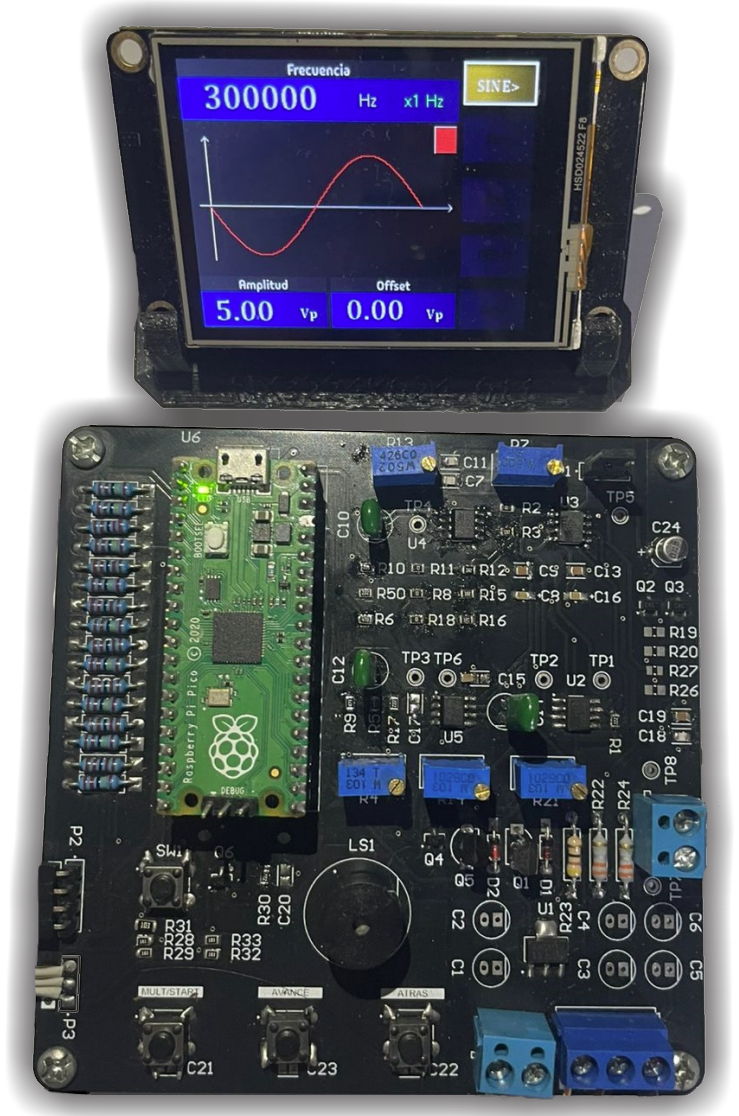
\includegraphics[height=1.2em]{Introduccion/img/dispositivo.png}}\hspace{0.3em}\thesection}
{0.5em}
{}
[\vspace{-0.5em}\color{teal}\rule{\linewidth}{2pt}]

\titleformat{\subsection}
{\normalfont\large\bfseries\color{teal}}{\thesubsection}{1em}{}
\titlespacing*{\subsection}{0pt}{0.5em}{0.5em}

\titleformat{\subsubsection}
{\normalfont\large\bfseries\color{teal}}{\thesubsubsection}{1em}{}
\titlespacing*{\subsubsection}{0pt}{0.5em}{0.5em}

% =========================================================
% ÍTEM CON IMAGEN (enumitem ya está en config.tex)
% =========================================================
\newcommand{\itemimage}{
\includegraphics[width=0.025\textwidth]{pic/items_control.png}}
\setlist[itemize]{label=\itemimage}

\begin{document}
	
	% =========================================================
	% CARÁTULA SIN ENCABEZADO
	% =========================================================
	% =========================================================
% CARÁTULA
% =========================================================
\begin{titlepage}
	\thispagestyle{empty} % sin encabezado ni pie
	
	\vspace*{-3cm}
	
	% --- Logos arriba ---
	\begin{minipage}[t]{0.49\textwidth}
		\raggedright
		
\includegraphics[width=3.2cm]{pic/unr-logo.png}
	\end{minipage}
	\begin{minipage}[t]{0.49\textwidth}
		\raggedleft
		
\includegraphics[width=5.3cm]{pic/FCEIA-logo.png}
	\end{minipage}
	
	\vspace{1cm}
	
	% --- Institución ---
	\begin{center}
		{\Large Universidad Nacional de Rosario \par}
		\vspace{0.15cm}
		{\large Facultad de Ciencias Exactas, Ingeniería y Agrimensura \par}
		\vspace{0.15cm}
		{\large Ingeniería Electrónica \par}
	\end{center}
	
	\vspace{2cm}
	
	% --- Título principal ---
	\begin{center}
		{\bfseries\LARGE Anteproyecto\par}
		\vspace{0.35cm}
		{\bfseries\Large Generador de Funciones Arbitrarias basado en DDS\par}
		\vspace{0.25cm}
		{\large \par}
	\end{center}
	
	\vspace{2cm}
	
	% --- Línea decorativa ---
	\noindent\rule{\textwidth}{1.2pt}
	
	\vspace{0.9cm}
	
	% --- Datos en dos columnas ---
	\noindent\makebox[\textwidth]{%
		\begin{minipage}[t]{0.49\textwidth}
			\raggedright
			{\bfseries Estudiante:}\par
			Agustín Zuliani, Legajo: Z-1183/5\par
			\vspace{0.6cm}
			{\bfseries Carrera:}\par
			Ingeniería Electrónica\par
		\end{minipage}%
		\hfill
		\begin{minipage}[t]{0.49\textwidth}
			\raggedleft
			{\bfseries Director:}\par
			Daniel Márquez\par
			\vspace{0.6cm}
			{\bfseries Asignatura / Proyecto:}\par
			Proyecto 1\par
		\end{minipage}%
	}
	
	\vspace{0.9cm}
	
	% --- Línea decorativa ---
	\noindent\rule{\textwidth}{1.2pt}
	
	\vfill
	
	% --- Pie ---
	\begin{center}
		Rosario, Santa Fe — 2025\par
	\end{center}
	
\end{titlepage}

	
	\newpage
	
	\tableofcontents
	\newpage
	
	\section{Introducción}
Un generador de formas de onda arbitrarias (AWG) permite generar funciones periódicas cargando puntos en un buffer y reproduciéndolos mediante un DAC a la frecuencia solicitada. La resolución depende de la profundidad del buffer y del DAC, afectando la frecuencia máxima alcanzable.

La idea de este proyecto consiste en la implementación de dicho generador de funciones basado en un microcontrolador relativamente nuevo \textbf{RP2040}. Este microcontrolador es de la familia \textit{Raspberry Pi}. A continuación puede verse una imagen preliminar de su pinout.

\begin{figure}[H]
	\centering
	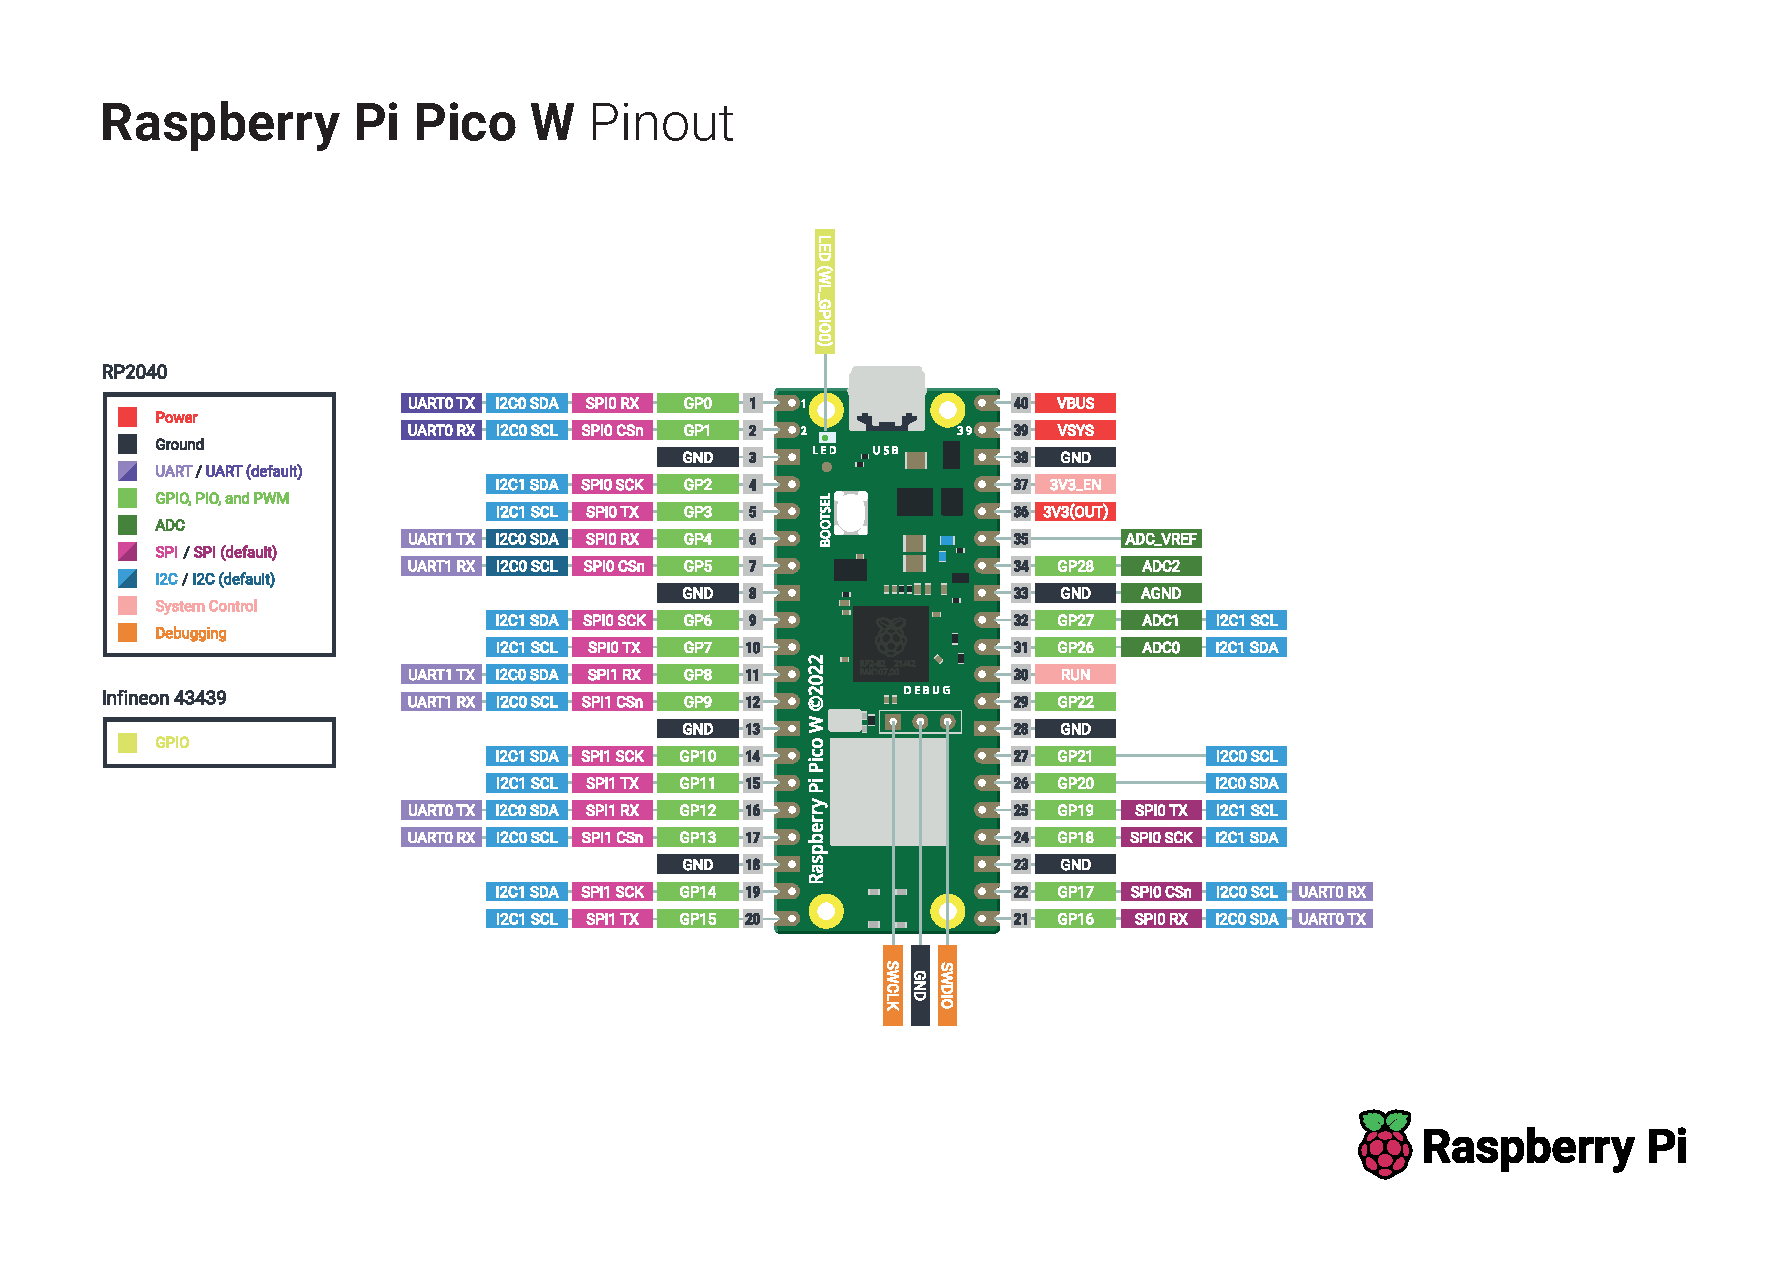
\includegraphics[width=\linewidth]{Introduccion/img/raspberry-pi-pico-w-pinout}
	\caption{Raspberry Pi Pico W Pinout.}
	\label{fig:raspberry-pi-pico-w-pinout}
\end{figure}

Como sabemos dentro del mercado de los microcontroladores existen una gran variedad de ellos. \textcolor{blue}{¿Porqué entonces elegimos este en particular?} El RP2040 posee un periférico en particular denominado PIO (Programable Input/Output), podríamos pensar a dicho periférico como un fragmento de FPGA en su idea central, dado que ambos te permiten crear un hardware a medida que se adapta a señales digitales que con periféricos existentes no es posible. La diferencia es que con una FPGA se define una lógica (por ejemplo utilizando flip-flops, FSMs, Sumadores, etc) y diciendo como estos deben conectarse. Con el PIO se programan unas máquinas de estados que ejecutan un conjunto de instrucciones para leer/generar señales de forma determinista y concurrente. Este microcontrolador posee un conjunto de 8 máquinas de estado. Al estar embebido dentro del propio microcontrolador permite manipularlo junto con otros periféricos dentro del mismo. En particular permite controlar los propios GPIOs. Entonces la idea detrás del Generador de Funciones consiste en producir un DAC (conversor de digital a analógico) que pueda actuar a altas velocidades. El proceso sería primero tener cargado en RAM cada punto de la señal a muestrear, luego transferirlo mediante DMA hacia el periférico PIO y que este mismo se encargue de producir el valor de tensión deseado habilitando o no salidas GPIOs mediante un DAC R2R (el cual puede verse en la figura ).

\begin{figure}[H]
	\centering
	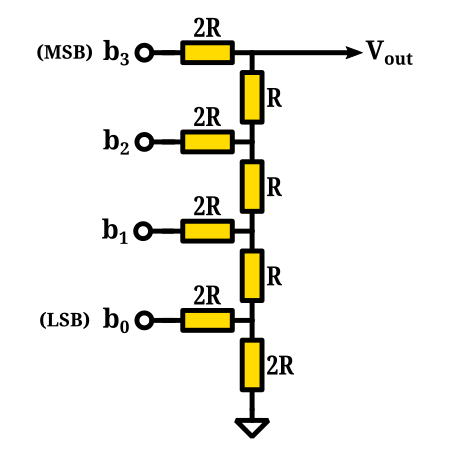
\includegraphics[width=0.5\linewidth]{Introduccion/img/r2r-4bits-2}
	\caption{DAC R-2R de 4 Bits. Este tipo de DAC permite tener un valor de tensión de acuerdo a la cantidad de bits habilitados y su ponderación. La resolución (mínima representación de valor de tensión) depende de la cantidad de bits. Con 4 bits y una alimentación de 3V3 la resolución es de 206 mV.}
	\label{fig:r2r-4bits-2}
\end{figure}

Este proyecto consiste en la continuación de un trabajo que se realizó en otras materias. Este proyecto base es el generador de funciones arbitrarias con dicho micro realizado con el conjunto de resistencias R-2R. La idea sería poder realizar un dispositivo completo con una mejora clara a nivel tecnológico. Partiendo de que la base de usar un DAC con resistencias R-2R se cambiarían por un sintetizador digital directo (DDS). En particular se quiere utilizar el AD9102 que tiene 12 bits de resolución a comparación de los 8 bits implementados en la versión anterior. También hay cierta mejoras respecto a la corriente máxima que permite a la salida del conector BNC, así como la impedancia de salida que sea de $50 \ \Omega$. Las versiones anteriores no dejaban de ser prototipos, la idea ahora es realizar un equipo completo en donde se tengan las placas de desarrollos diseñadas, una fuente de alimentación conmutada conectada a 220 Vac y una carcasa en 3D o en su caso en chapa.

\section{Motivación}
La motivación para realizar el proyecto comenzó como parte de un trabajo práctico de la materia \textit{Dispositivos y Circuitos Electrónicos IV} donde se realizó una primera versión del desarrollo. El trabajo únicamente consistía en generar la señal con el DAC 2-2R y eligiendo mediante una pantalla TFT el valor de la frecuencia de salida. Debido al tiempo limitado el hardware se realizó lo mencionado, quedando como futura mejora la implementación de un control de acondicionamiento de señal, permitiendo variar el amplitud máxima, offset y tipo de señal. Por el lado del firmware de la primera versión un Framework que permite modelar máquinas de estados jerárquicas. Este Framework se llama \textbf{Quantum Leaps}. A continuación se muestra una foto de la primera versión realizada en una placa perforada y luego la MEF implementada.

\begin{figure}[H]
	\centering
	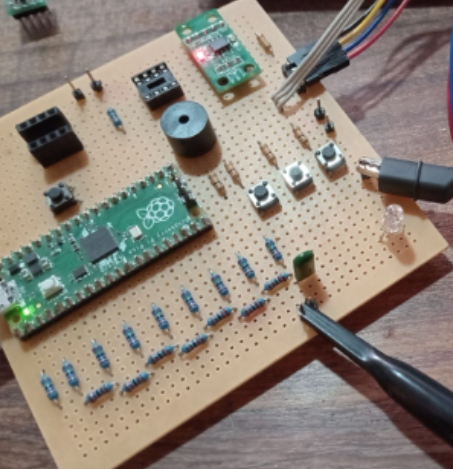
\includegraphics[width=0.5\linewidth]{Introduccion/img/1raVersionPlaca}
	\caption{Primera versión de la placa de desarrollo, realizada con una placa perforada.}
	\label{fig:1raversionplaca}
\end{figure}

\begin{figure}[H]
	\centering
	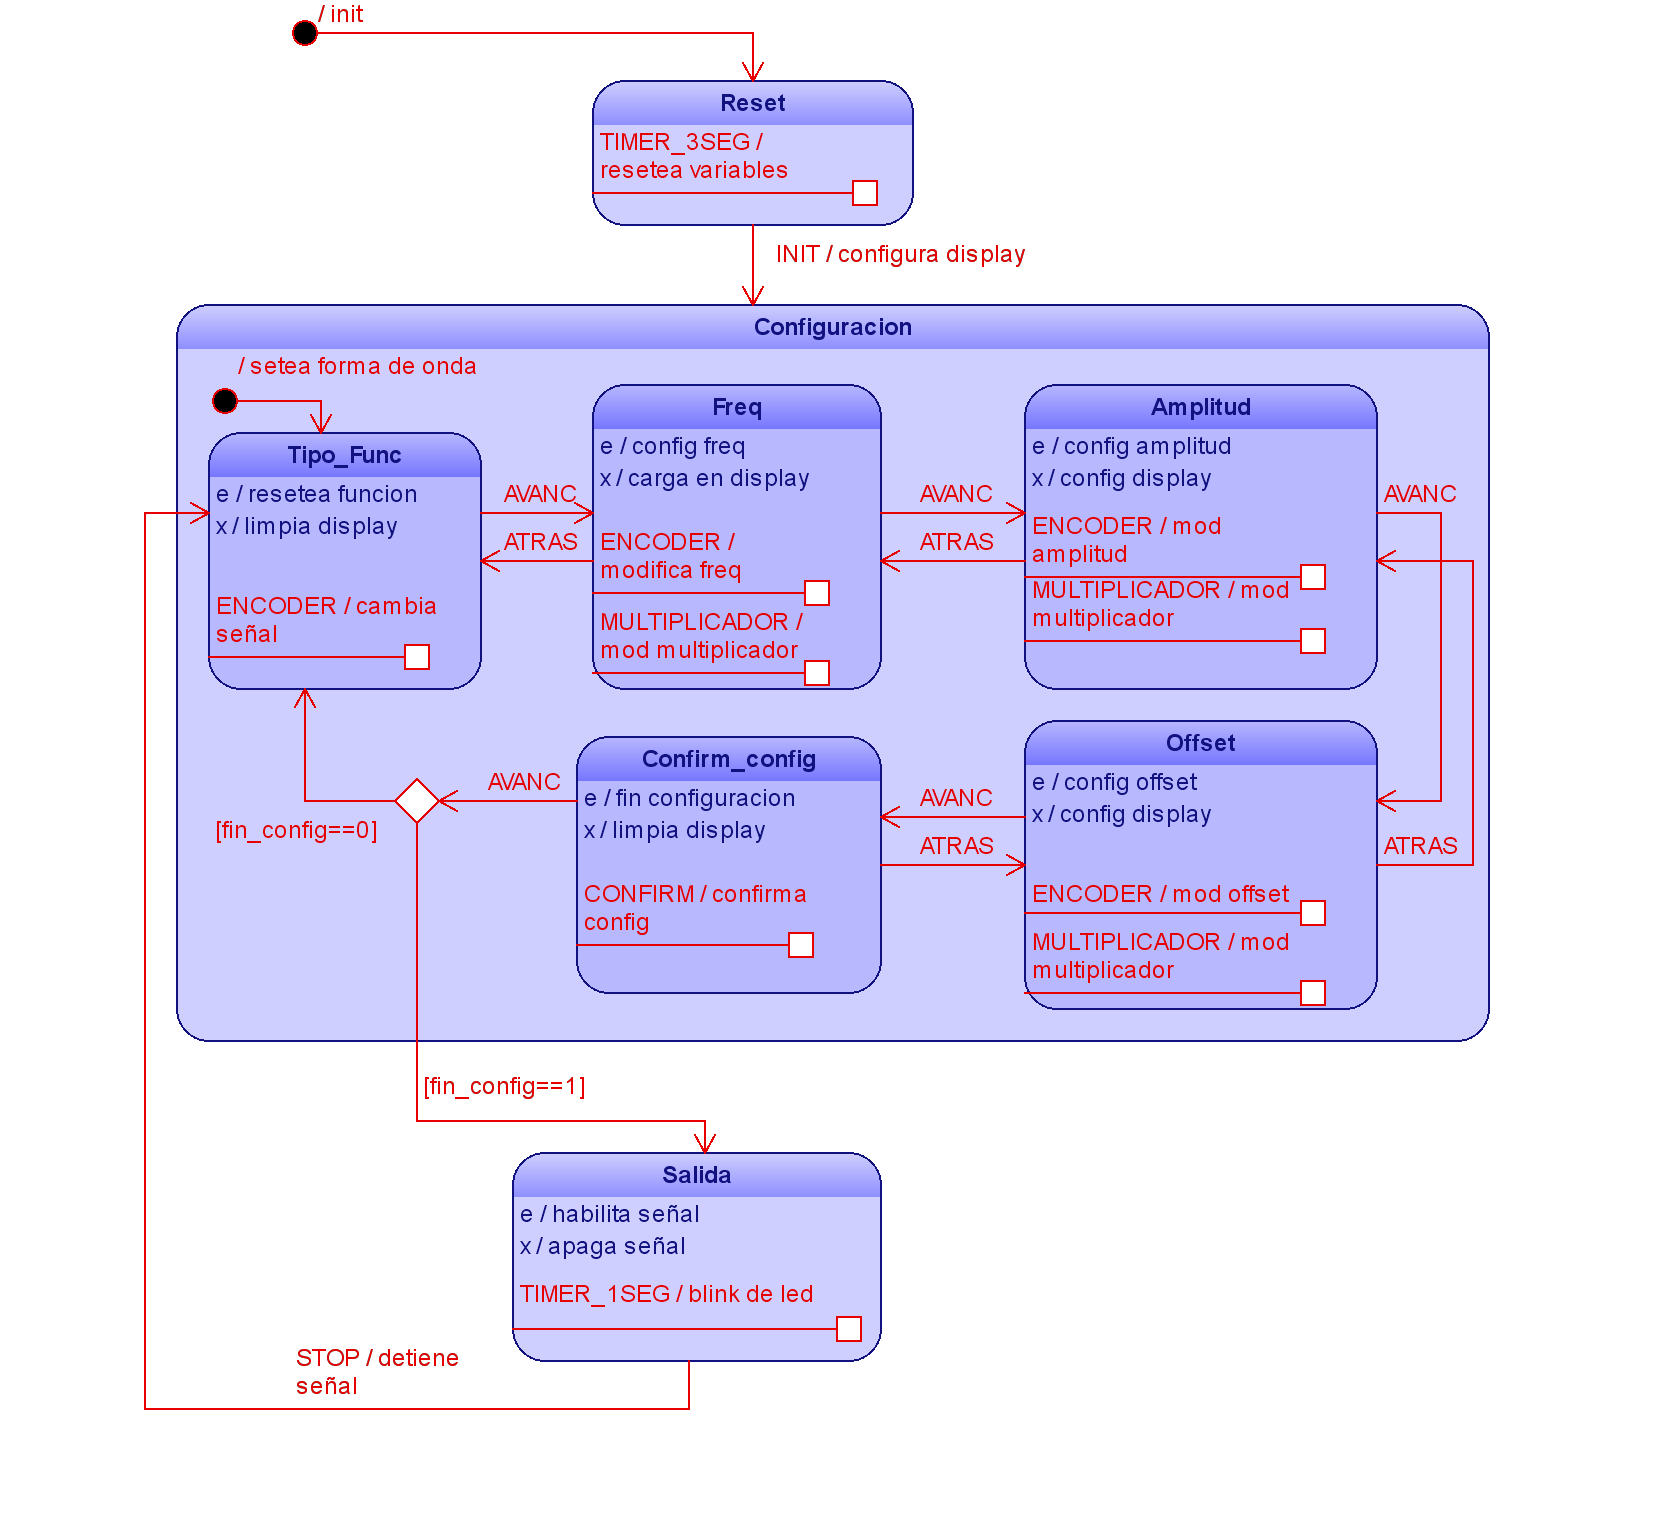
\includegraphics[width=0.7\linewidth]{Introduccion/img/SM_of_Awg}
	\caption{Máquina de estado implementada en el modelado.}
	\label{fig:smofawg}
\end{figure}

A grandes rasgos se pueden observar tres estados principales (\textbf{Reset},\textbf{Configuración} y \textbf{Salida}). Luego dentro de \textit{Configuración} se tienen sus respectivos sub-estados. La idea detrás de esta MEF es permitir que el usuario permita una configuración de cada parámetro del generado de funciones realizado observando los cambios en una pantalla TFT de 2.4 in. Tal como se mencionó solamente permitía configurarse la frecuencia en la primera versión del proyecto, por lo que los sub-estados \textit{Amplitud, Offset} estaban deshabilitados.

Posteriormente dicho proyecto fue continuado en la materia de \textit{Sistemas Embebidos Avanzados II}. Uno de los contenidos de dicha materia es programación en \textit{Sistemas Operativos en Tiempo Real} ()\textbf{RTOS}). En particular se utilizó el conocido \textbf{FreeRTOS}. Como trabajo final para la materia se decidió continuar con el proyecto ya mencionado, agregándole en este caso el \textbf{FreeRTOS} junto con la máquina de estado que ya formaba parte del proyecto base. Como mejora a nivel de Hardware se procedió a realizar una PCB de doble capa, la cual se mandó a realizar a China en \textbf{JLCPCB}. Se puede visualizar a continuación una imagen de dicha PCB.

\begin{figure}[H]
	\centering
	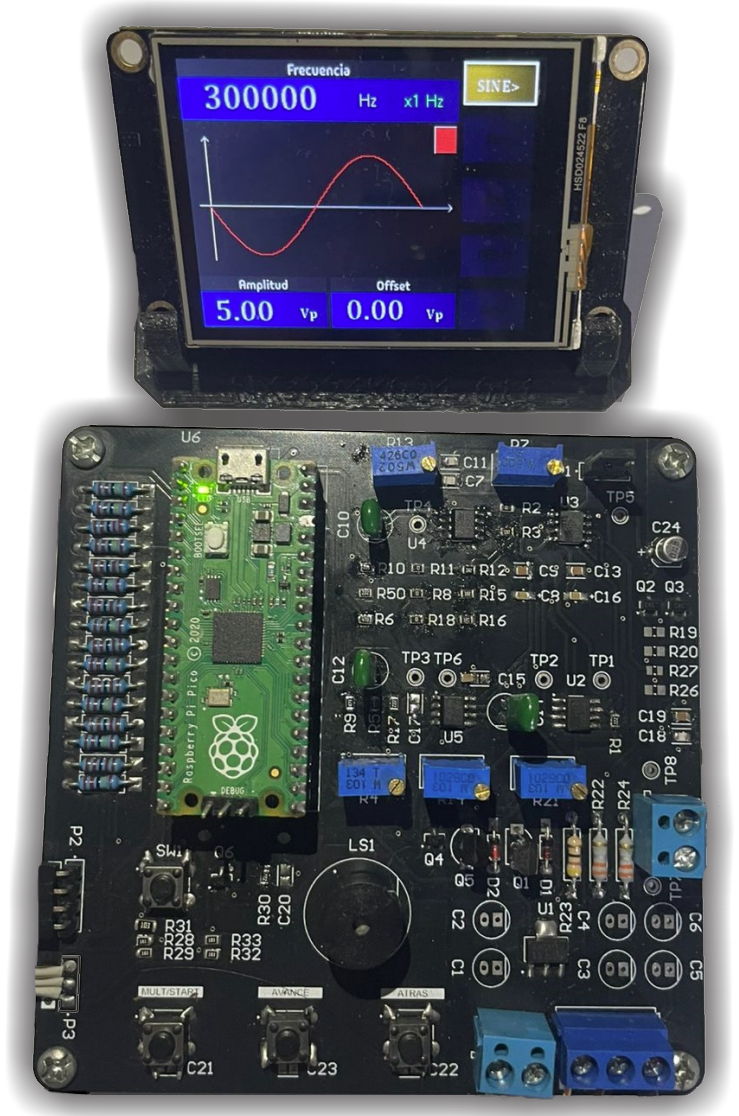
\includegraphics[width=0.6\linewidth]{Introduccion/img/dispositivo}
	\caption{Segunda versión de la PCB del generador de funciones Arbitrario.}
	\label{fig:dispositivo}
\end{figure}

En esta versión ya se puede ver claramente las distintas partes que componen el circuito en la capa Top. Por un lado se tiene el DAC R-2R junto con el micro. Por el lado derecho se tiene la lógica de control. Dentro de estas mejoras de Hardware ya se incluyó la posibilidad de generar una amplificación de la señal, junto con el offset respectivo. Para poder realizar esto se utilizó un potenciómetro digital, señales PWM (junto con filtros \textit{Pasa Bajos Activos}) y operacionales. Dado que dentro de las características solicitadas se había la mencionado la posibilidad de poder generar señales de hasta 1 MHz, aparecía una limitación en la ganancia máxima a dicha frecuencia y en el Slew Rate máximo en el promedio de los Operacionales que se venden en el mercado local. De esta forma se procedió a una investigación sobre los Amplificadores Operacionales disponibles en Mercado Libre que permitieran tener una Ganancia considerable a alta frecuencia y además un elevado Slew Rate. Luego de este proceso se optó por el LM6172 que tiene un ancho de banda de 100 MHz y un Slew Rate 3000 V/$\mu$S.

Para poder visualizar la información que el usuario va configurando se utilizó una pantalla TFT Nextion de 2.4 in. Para esto posee un enconder rotativo de 20 vueltas (no se observa en la imagen) y pulsadores para avanzar, retroceder y cambiar el multiplicador (de tensión, frecuencia y offset). Una vez que el usuario termina de configurar la salida luego esta señal se carga en un buffer y se procede a muestrear a través de los periféricos \textbf{DMA} y \textbf{PIO}. En particular se muestra un ejemplo de una salida senoidal con 10 Vpp y 50 KHz.

\begin{figure}[H]
	\centering
	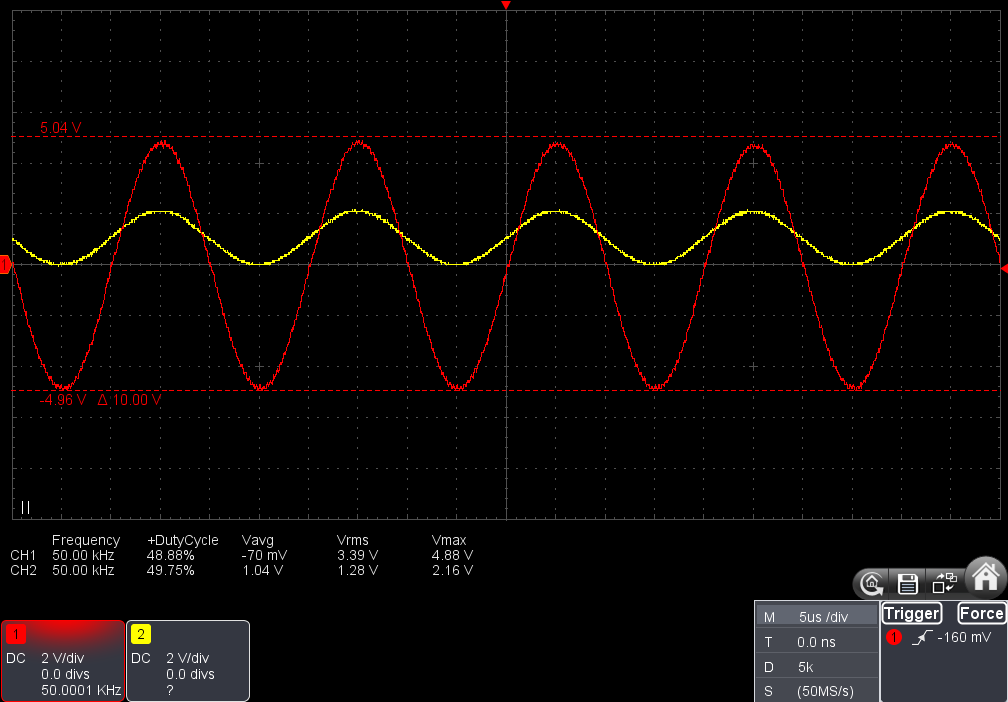
\includegraphics[width=0.7\linewidth]{Introduccion/img/10VPP_50KHZ_SENOIDAL}
	\caption{Señal Senoidal con una amplitud de 10 Vpp y 50 KHz.}
	\label{fig:10vpp50khzsenoidal}
\end{figure}

En amarillo se puede observar la señal que sale desde el DAC R-2R y en rojo la señal amplificada y con offset nulo.
%	\section{Alcance y Objetivos}
La intención de este proyecto consiste en la realización de dicho \textit{Generador de Funciones Arbitrarias} para esto mismo se proponen ciertas características para validar la calidad del dispositivo realizado:

\begin{itemize}
	\item $V_{opp} = $ 10 Vpp.
	\item $V_{in} = $ 85 a 265 VAC.
	\item $I_{o}$ = 20 mA.
	\item 
\end{itemize}
	\subsection{Equipos de referencia en el mercado}
Los generadores de funciones arbitrarias orientados a aplicaciones de laboratorio y enseñanza presentan un conjunto de características técnicas comunes que definen este segmento tecnológico. En términos generales, estos equipos ofrecen:

\begin{itemize}
	\item Rango de frecuencia senoidal típico entre 10 MHz a 30 MHz.
	\item Resolución vertical comprendida entre 12 y 14 bits.
	\item Impedancia de salida nominal de 50 $\Omega$.
	\item Amplitud máxima de hasta 20 Vpp en carga de alta impedancia.
	\item Offset DC ajustable.
	\item Control de fase relativo entre canales.
	\item Formas de onda convencionales (senoidal, cuadrada, triangular) y formas arbitrarias previamente cargadas.
\end{itemize}

Adicionalmente, suelen incorporar funcionalidades como barrido de frecuencia (sweep), generación por ráfagas (burst), modulación básica (AM/FM) y sincronización entre canales.

En cuanto a la interfaz de usuario, es habitual la presencia de pantalla gráfica, control rotativo incremental y conectividad mediante interfaces digitales como USB o LAN para control remoto.

El presente desarrollo se posiciona dentro de este rango tecnológico, tomando como referencia las prestaciones comúnmente ofrecidas en el segmento de media prestación.

%\subsubsection{UNIT-T Utg962e 60 Mhz:} Se trata de un generador de funciones arbitrario de 60 MHz. Posee algunas características que se destacan a continuación:
%
%\begin{itemize}
%	\item \textbf{Canales:} 2
%	\item \textbf{Frecuencia máxima:} 60\,MHz
%	\item \textbf{Tasa de muestreo (Sampling rate):} 200\,MS/s
%	\item \textbf{Resolución vertical:} 14\,bits
%	\item \textbf{Formas de onda:} Senoidal, cuadrada, pulso, rampa, ruido, DC y arbitraria
%	\item \textbf{Modos de barrido (Sweep):} Logarítmico y lineal
%	
%	\item \textbf{Características de frecuencia:}
%	
%	\begin{itemize}\renewcommand{\labelitemii}{$\bullet$}
%		\item Senoidal: $1\,\mu\text{Hz}$ -- $60\,\text{MHz}$
%		\item Cuadrada: $1\,\mu\text{Hz}$ -- $20\,\text{MHz}$
%		\item Rampa: $1\,\mu\text{Hz}$ -- $400\,\text{kHz}$
%		\item Pulso: $1\,\mu\text{Hz}$ -- $20\,\text{MHz}$
%		\item Arbitraria: $1\,\mu\text{Hz}$ -- $10\,\text{MHz}$
%		\item Resolución en frecuencia: $1\,\mu\text{Hz}$
%	\end{itemize}
%	
%	\item \textbf{Características de salida:}
%	\begin{itemize}\renewcommand{\labelitemii}{$\bullet$}
%		\item Impedancia: $50\,\Omega$ / High~Z
%		\item Rango de amplitud: $1\,\text{mVpp}$ -- $10\,\text{Vpp}$ (a $50\,\Omega$);\;
%		$2\,\text{mVpp}$ -- $20\,\text{Vpp}$ (High~Z)
%		\item Rango de offset DC (AC+DC): $\pm 5\,\text{V}$ (a $50\,\Omega$);\; $\pm 10\,\text{V}$ (High~Z)
%		\item Resolución de amplitud: $1\,\text{mV}$
%	\end{itemize}
%	
%	\item \textbf{Alimentación:} 100--240\,VAC, 50/60\,Hz
%	\item \textbf{Display:} 4.3'' TFT LCD (480$\times$272)
%\end{itemize}
%
%\begin{figure}[H]
%	\centering
%	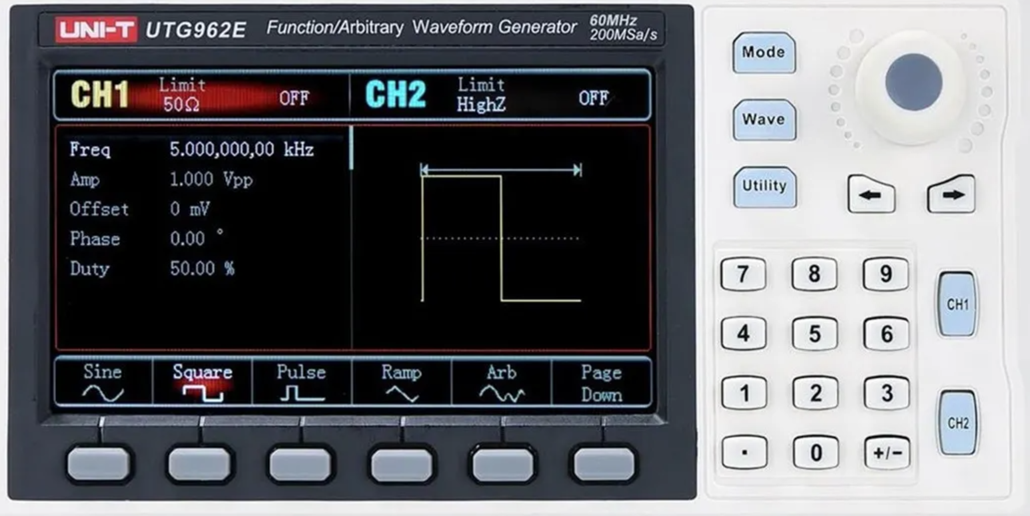
\includegraphics[width=0.7\linewidth]{Comparacion/img/unit-t}
%	\caption{Imagen ilustrativa del Generador de Funciones Arbitrarias de UNIT-T.}
%	\label{fig:unit-t}
%\end{figure}
%
%\subsubsection{OWON DGE2035:}
%Generador de funciones/arbitrario de \textbf{2 canales} con frecuencia máxima de \textbf{35\,MHz}. Sus características principales son:
%
%\begin{itemize}
%	\item \textbf{Canales:} 2
%	\item \textbf{Frecuencia máxima (salida):} 35\,MHz
%	\item \textbf{Tasa de muestreo (Sampling rate):} 125\,MSa/s
%	\item \textbf{Resolución vertical:} 14\,bits
%	\item \textbf{Longitud de forma arbitraria:} hasta 8K puntos
%	\item \textbf{Formas de onda:} senoidal, cuadrada, pulso, rampa y ruido; además incluye \textbf{150} formas arbitrarias predefinidas y permite forma arbitraria definida por el usuario
%	\item \textbf{Características de frecuencia (resolución en frecuencia: 1\,$\mu$Hz):}
%	\begin{itemize}\renewcommand{\labelitemii}{$\bullet$}
%		\item Senoidal: $1\,\mu\text{Hz}$ -- $35\,\text{MHz}$
%		\item Cuadrada: $1\,\mu\text{Hz}$ -- $15\,\text{MHz}$
%		\item Pulso: $1\,\mu\text{Hz}$ -- $15\,\text{MHz}$
%		\item Rampa: $1\,\mu\text{Hz}$ -- $1\,\text{MHz}$
%		\item Arbitraria: $1\,\mu\text{Hz}$ -- $10\,\text{MHz}$
%	\end{itemize}
%	\item \textbf{Modulación:} AM, FM, PM, FSK, Sweep y Burst
%	\item \textbf{Interfaz/Control:} USB Host; compatible con SCPI y LabVIEW
%	\item \textbf{Display:} TFT 3.6'' (480$\times$272)
%\end{itemize}
%
%\begin{figure}[H]
%	\centering
%	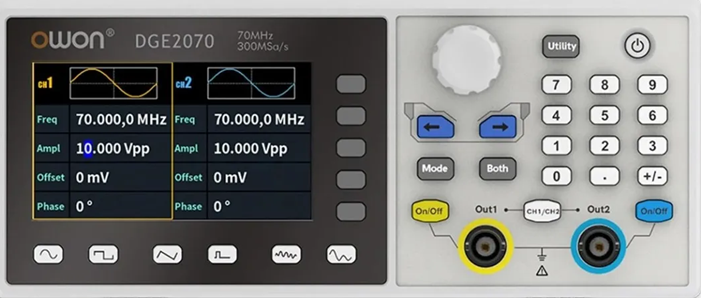
\includegraphics[width=0.7\linewidth]{Comparacion/img/owon}
%	\caption{Generador de Funciones Arbitrarias de la marca OWON.}
%	\label{fig:owon}
%\end{figure}
%
%\subsubsection{Generador DDS FeelElec FY6900-20M (20\,MHz):}
%Generador de funciones/arbitrario \textbf{de dos canales} basado en \textbf{DDS}. Especificaciones principales:
%
%\begin{itemize}
%	\item \textbf{Canales:} 2
%	\item \textbf{Tecnología:} DDS (Direct Digital Synthesizer)
%	\item \textbf{Tasa de muestreo (Sampling rate):} 250\,MSa/s
%	\item \textbf{Resolución vertical:} 14\,bits
%	\item \textbf{Longitud de forma arbitraria:} 8192 puntos (8K) \,$\times$\,14\,bits
%	\item \textbf{Resolución mínima de frecuencia:} 1\,$\mu$Hz
%	
%	\item \textbf{Rangos de frecuencia (modelo 20\,MHz):}
%	\begin{itemize}\renewcommand{\labelitemii}{$\bullet$}
%		\item Senoidal: 0--20\,MHz
%		\item Cuadrada: 0--15\,MHz
%		\item Triangular / Rampa: 0--10\,MHz
%		\item Pulso: 0--10\,MHz \;(\textbf{ancho mínimo de pulso:} 20\,ns)
%		\item Arbitraria: 0--10\,MHz
%	\end{itemize}
%	
%	\item \textbf{Formas de onda:} Seno, cuadrada, rectangular (duty ajustable), pulso, triangular/rampa,
%	diente de sierra, DC, ruido, ECG, y formas arbitrarias (predefinidas y definidas por el usuario)
%	
%	\item \textbf{Salida:}
%	\begin{itemize}\renewcommand{\labelitemii}{$\bullet$}
%		\item Impedancia de salida: 50\,$\Omega$ (típica, $\pm 10\%$)
%		\item Resolución de amplitud: 1\,mV
%		\item Rango de amplitud (Vpp) según frecuencia:
%		\begin{itemize}
%			\item $f \le 5\,\text{MHz}$: 1\,mVpp -- 24\,Vpp
%			\item $5\,\text{MHz} < f \le 10\,\text{MHz}$: 1\,mVpp -- 20\,Vpp
%			\item $10\,\text{MHz} < f \le 20\,\text{MHz}$: 1\,mVpp -- 10\,Vpp
%			\item $f > 20\,\text{MHz}$: 1\,mVpp -- 5\,Vpp
%		\end{itemize}
%	\end{itemize}
%	
%	\item \textbf{Offset DC:}
%	\begin{itemize}\renewcommand{\labelitemii}{$\bullet$}
%		\item Rango: $\pm 12$\,V (hasta 20\,MHz), $\pm 2.5$\,V (por encima de 20\,MHz)
%		\item Resolución: 1\,mV
%	\end{itemize}
%	
%	\item \textbf{Fase:} 0--359.99$^\circ$ \;(\textbf{resolución:} 0.01$^\circ$)
%	\item \textbf{Duty cycle (rectangular):} 0.01\%--99.99\% \;(\textbf{resolución:} 0.01\%)
%	\item \textbf{Modulación:} AM, FM, PM, ASK, FSK, PSK
%	\item \textbf{Sweep:} lineal y logarítmico (frecuencia, amplitud, offset y duty)
%\end{itemize}
%
%\begin{figure}[H]
%	\centering
%	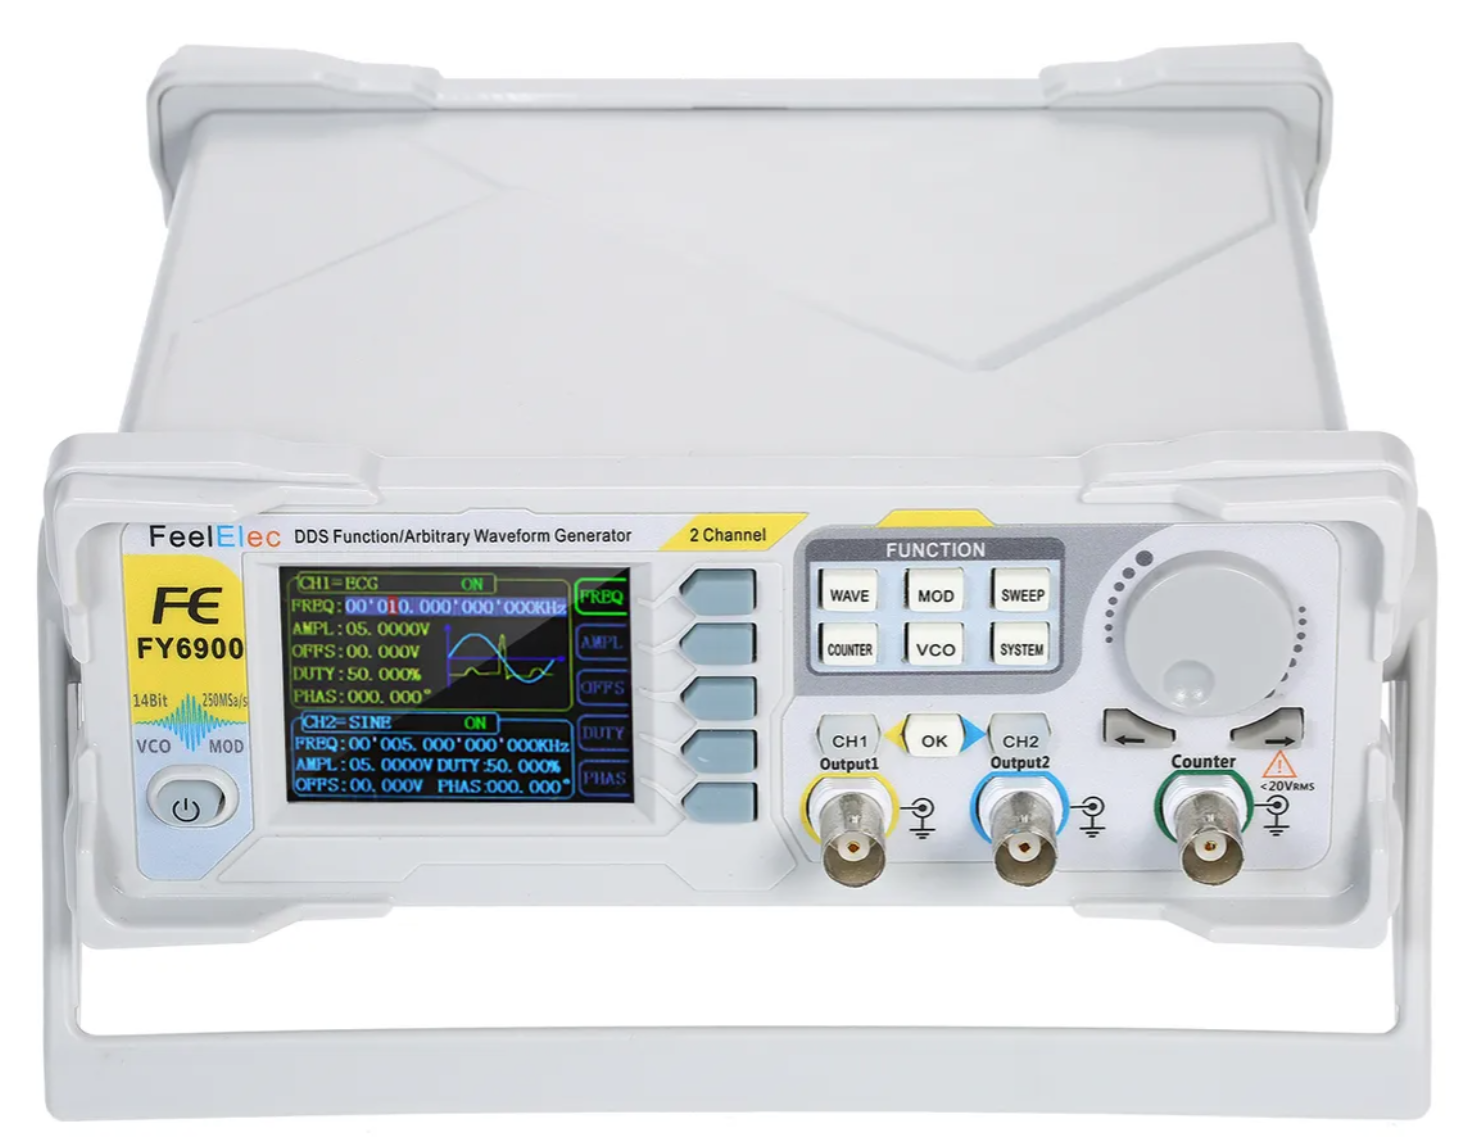
\includegraphics[width=0.7\linewidth]{Comparacion/img/Gaf-chino}
%	\caption{Generador de Funciones de marca FeelElec.}
%	\label{fig:gaf-chino}
%\end{figure}
	\section{Características del equipo}
A fin de definir el alcance del desarrollo y permitir la verificación objetiva del desempeño del instrumento, se establecen a continuación las especificaciones técnicas del equipo. Estas especificaciones constituyen los requisitos mínimos a cumplir y permiten comparar el resultado obtenido con instrumentos equivalentes del segmento de laboratorio y enseñanza.

\subsection{Configuración general}

\begin{itemize}
	\item \textbf{Cantidad de canales:} 2 canales de salida independientes y sincronizables.
\end{itemize}

\subsection{Especificaciones de alimentación}

La fuente de alimentación deberá permitir el correcto funcionamiento del sistema en las condiciones nominales de operación, incluyendo la provisión de rieles de tensión para las etapas digitales y analógicas.

\begin{itemize}
	\item \textbf{Rango de tensión de entrada:} $V_{ac}$ = 85 a 265 Vrms (alimentación universal).
	\item \textbf{Potencia máxima de entrada:} $P_{in,max}$ = 70 W.
\end{itemize}

\subsection{Especificaciones de forma de onda}

Se definen a continuación las especificaciones eléctricas mínimas de salida del instrumento:

\begin{itemize}
	\item \textbf{Tensión pico a pico máxima:} $V_{pp,max} =$ 20 Vpp en High-Z y 10 Vpp en 50 $\Omega$.
	\item \textbf{Tensión de pico máxima:} $V_{p,max} =$ 15 V en High-Z y 7.5 V en 50 $\Omega$.
	\item \textbf{Resolución de amplitud:} $\leq 100$ mVp.
	\item \textbf{Corriente máxima de salida:} $I_{o,max} \geq 100$ mA.
	\item \textbf{Impedancia de salida:} $Z_o = 50\,\Omega$.
	\item \textbf{Frecuencia máxima de salida:} $f_{max} \simeq$ 15 MHz (senoidal), 10 MHz (cuadrada/triangular) y 10 MHz (arbitraria).
	\item \textbf{Resolución de frecuencia:} $\leq 1$ Hz.
	\item \textbf{Generación arbitraria:} la forma arbitraria deberá permitir al menos $N \ge 16$ muestras por período a la frecuencia máxima especificada.
\end{itemize}

\subsection{Formas de onda disponibles}
El instrumento deberá permitir la generación de las siguientes formas de onda en cada canal de salida:

\begin{itemize}
	\item \textbf{Senoidal}
	\item \textbf{Cuadrada}, con ciclo de trabajo ajustable
	\item \textbf{Triangular}
	\item \textbf{Diente de sierra}, ascendente y descendente
	\item \textbf{Forma arbitraria} definida por el usuario
	\item \textbf{Señal continua (DC)}
\end{itemize}

Cada forma de onda deberá ser configurable en términos de frecuencia, amplitud y offset dentro de los rangos especificados en las subsecciones correspondientes.

\subsection{Interfaz de usuario}

\begin{itemize}
	\item \textbf{Pantalla gráfica:} display gráfico integrado para visualización de parámetros y forma de onda.
	\item \textbf{Método de control:} encoder rotativo incremental y pulsadores dedicados.
\end{itemize}

\subsection{Conectividad}

El instrumento deberá incorporar interfaces de comunicación destinadas a su integración con sistemas externos.

\begin{itemize}
	\item \textbf{Interfaz USB:}
	\begin{itemize}[label=\textbullet]
		\item Compatible con estándar USB 1.1 o superior.
		\item Comunicación serial virtual (CDC o equivalente).
		\item Soporte para actualización de firmware.
	\end{itemize}
	
	\item \textbf{Interfaz Ethernet:}
	\begin{itemize}[label=\textbullet]
		\item Compatibilidad con estándar 10/100 Mbps.
		\item Soporte para comunicación TCP/IP.
	\end{itemize}
\end{itemize}

\section{Arquitectura de implementación}
Con el fin de cumplir con las especificaciones definidas en la Sección 3, se propone una arquitectura modular dividida en dos grandes bloques: \textbf{Hardware} y \textbf{Firmware}.

\subsection{Arquitectura de Hardware}
El sistema se organiza en tres placas principales:

\begin{itemize}
	\item \textbf{Placa de Control}
	\item \textbf{Placa de Alimentación}
	\item \textbf{Placa de Panel Frontal}
\end{itemize}

\paragraph{Placa de Control:} integra los siguientes bloques funcionales (Figura \ref{fig:awgdds}):

\begin{itemize}[label=\textbullet]
	\item Núcleo de síntesis DDS.
	\item Unidad de control digital (microcontrolador).
	\item Etapa de conversión corriente–tensión diferencial.
	\item Conversión diferencial a simple.
	\item Control de amplitud (ajuste grueso y fino).
	\item Etapa de offset DC.
	\item Amplificación final y adaptación a 50 $\Omega$.
	\item Generación de reloj.
	\item Memoria no volátil.
	\item Etapa de alimentación y filtrado.
	\item Comunicación USB y/o LAN Ethernet.
	\item Comunicación con panel frontal.
\end{itemize}

\paragraph{Placa de alimentación:} provee los rieles simétricos y digitales necesarios para el correcto funcionamiento de las etapas analógicas y de control (Figura \ref{fig:panelalimentaciondds}).

\paragraph{Placa de panel frontal:} permite la interacción con el usuario final, manipulando y visualizando los diferentes periféricos.

%\begin{figure}[H]
%	\centering
%	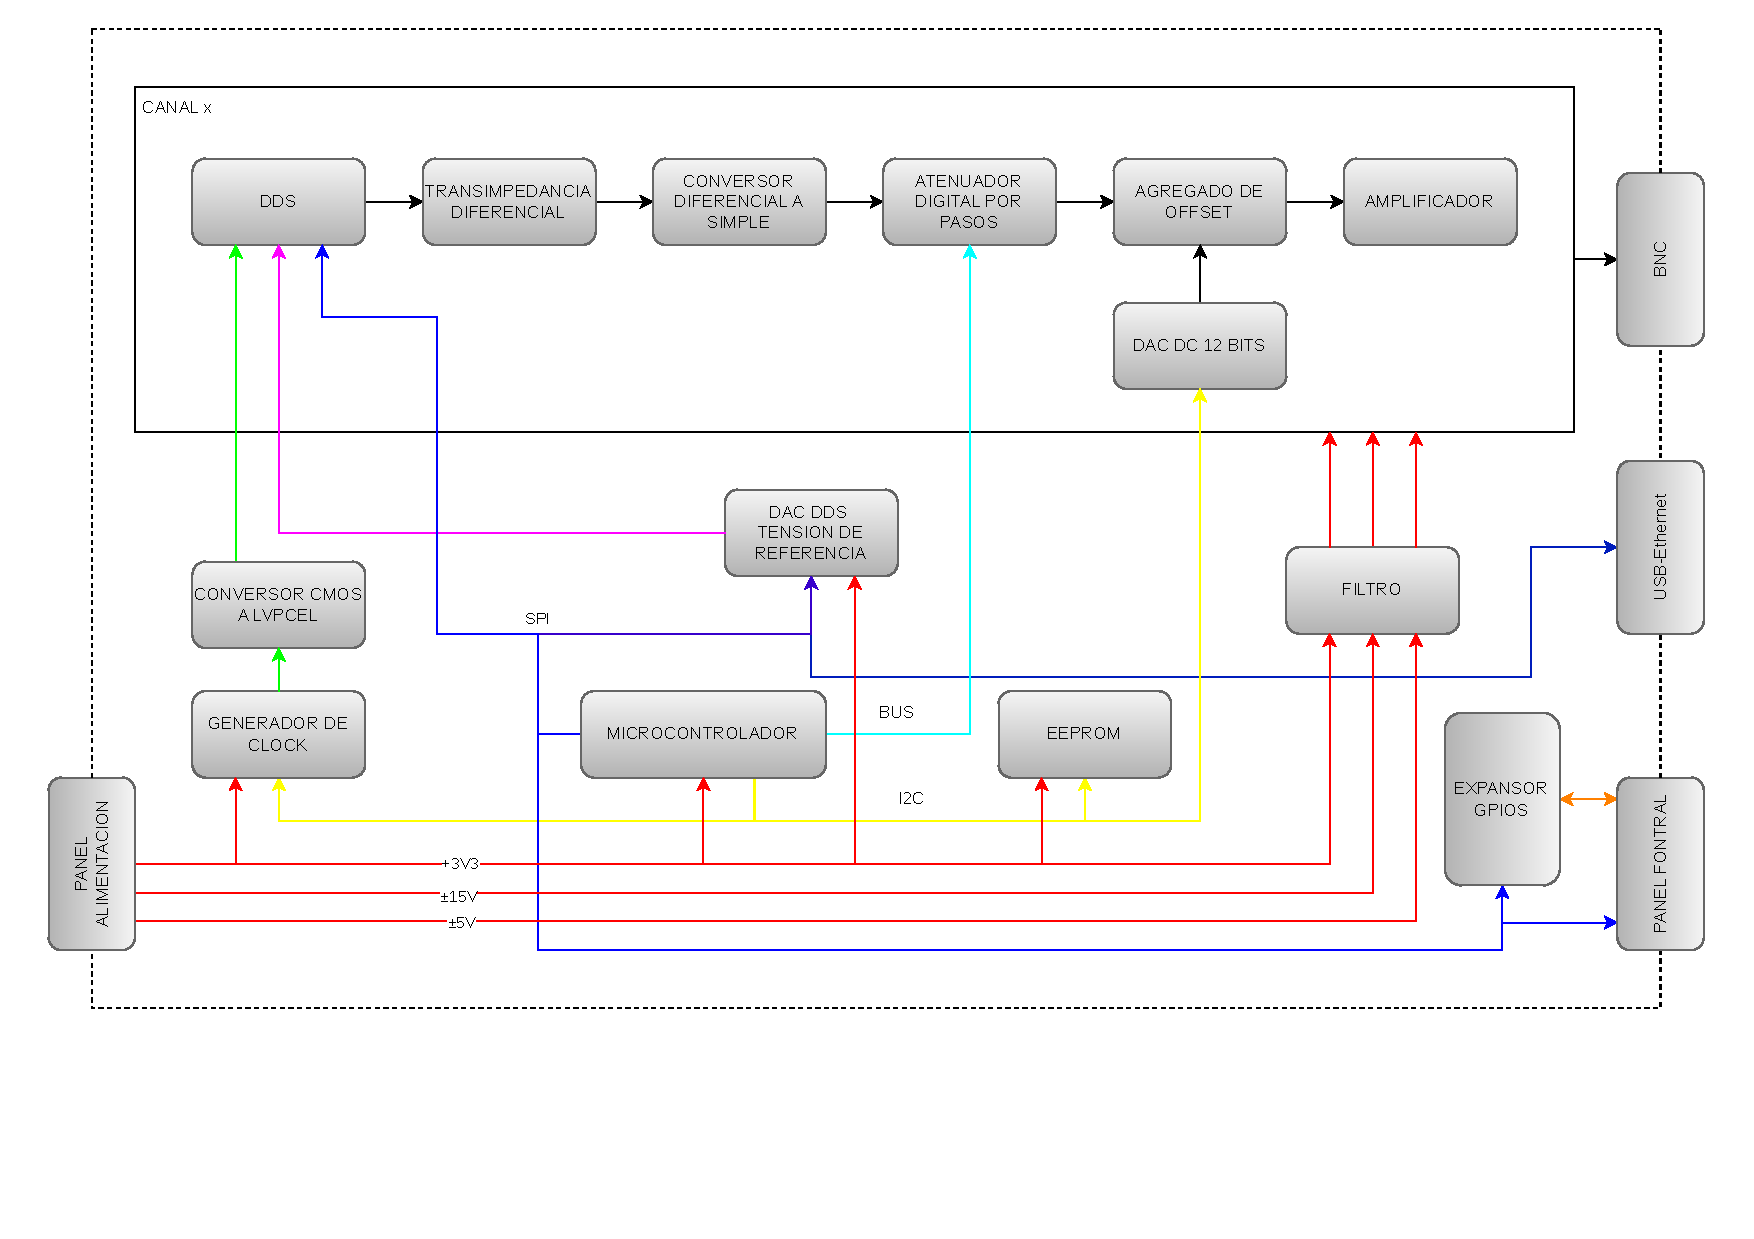
\includegraphics[width=0.8\linewidth]{img/AWG_DDS.pdf}
%	\caption{Diagrama en bloques del Hardware del Generador de Funciones Arbitrarias de la Placa de Control.}
%	\label{fig:awgdds}
%\end{figure}

\begin{sidewaysfigure}
	\centering
	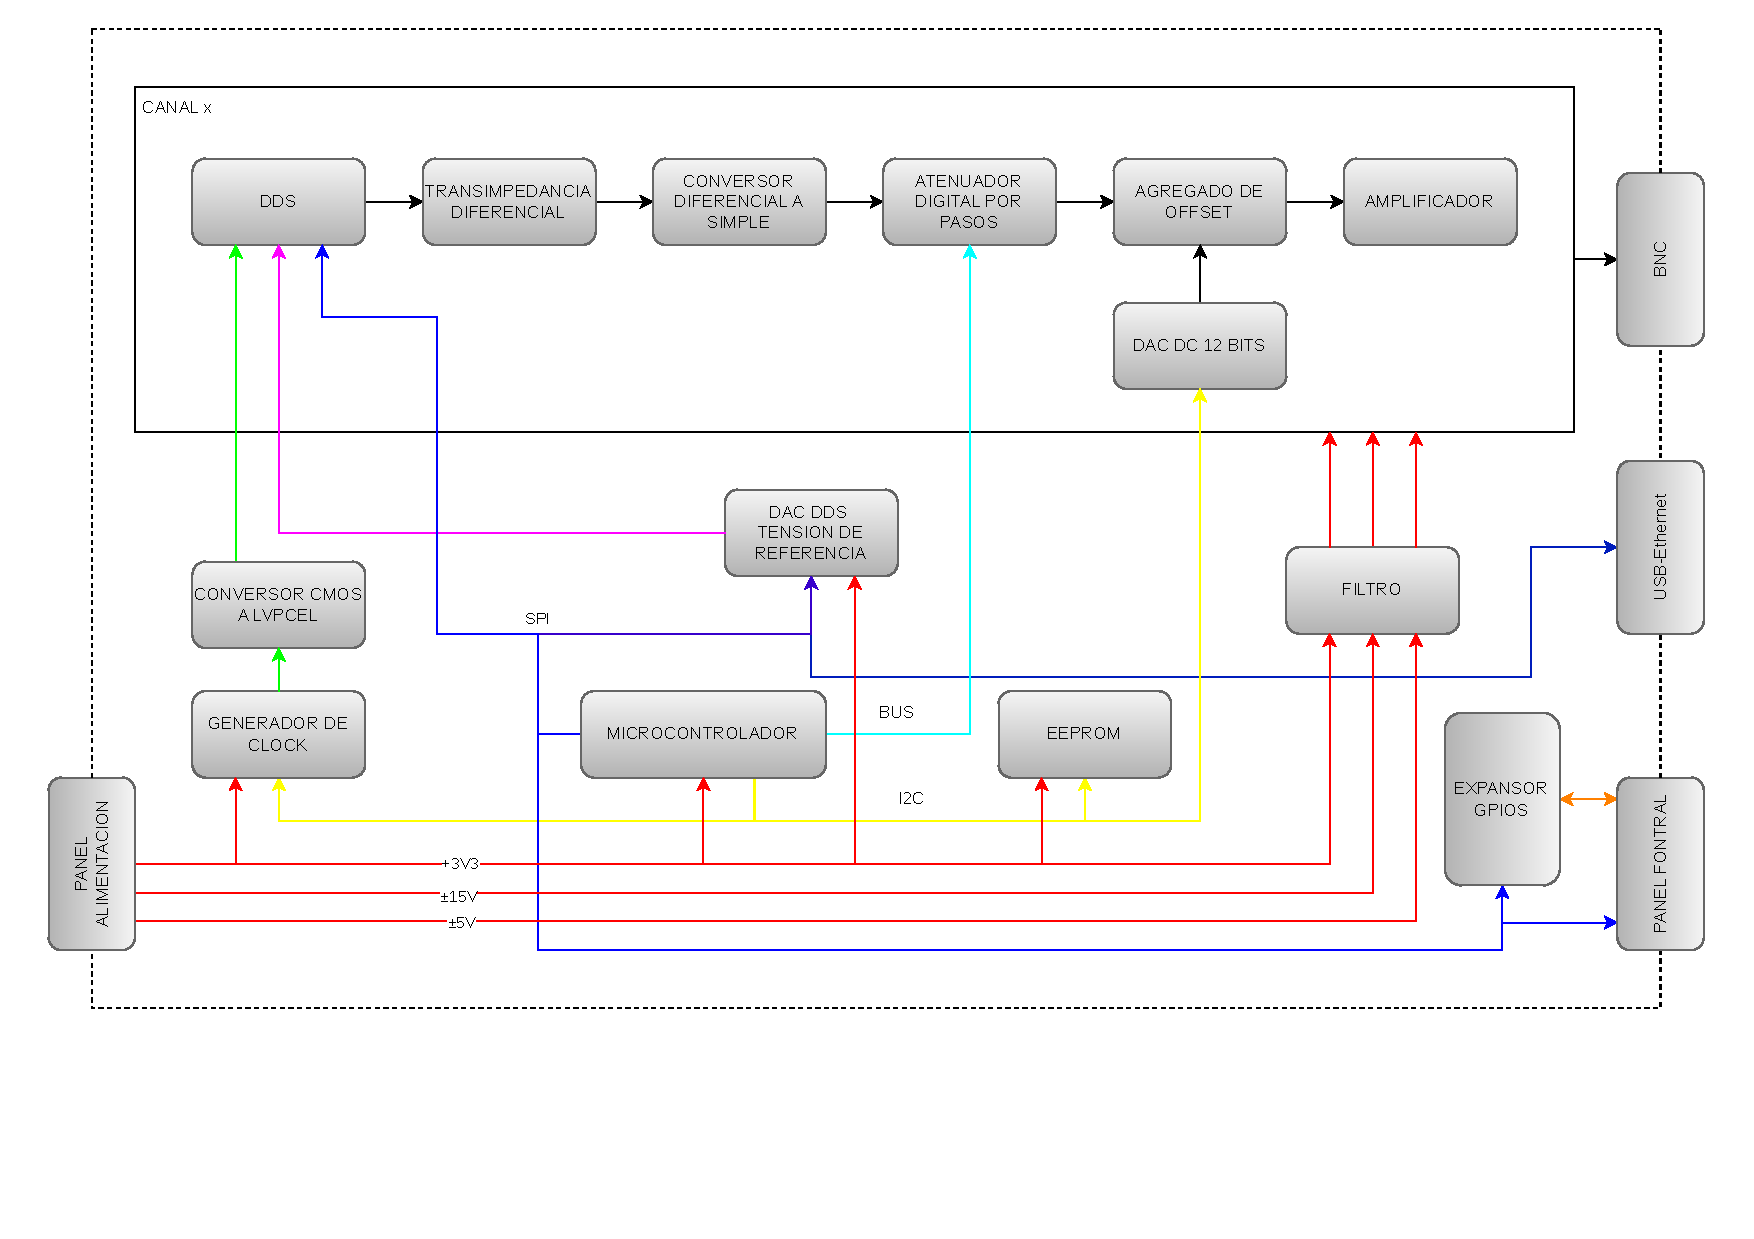
\includegraphics[width=\textheight]{img/AWG_DDS.pdf}
	\caption{Diagrama en bloques del Hardware del Generador de Funciones Arbitrarias de la Placa de Control.}
	\label{fig:awgdds}
\end{sidewaysfigure}


\begin{figure}[H]
	\centering
	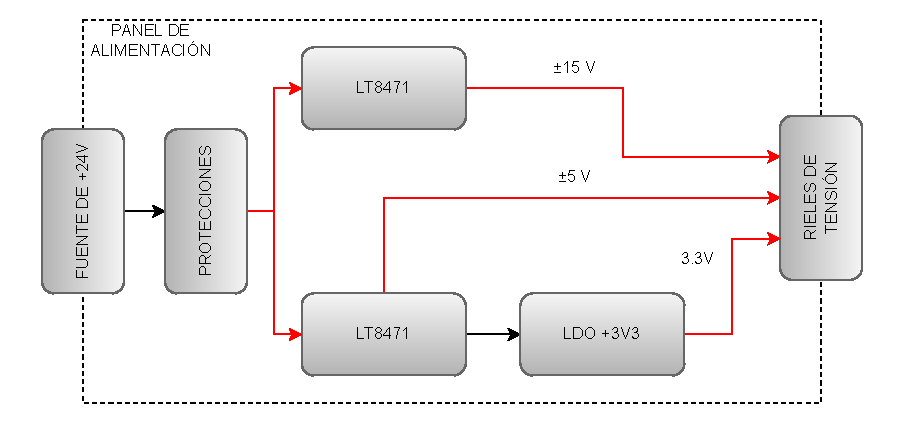
\includegraphics[width=0.7\linewidth]{img/PanelAlimentacionDDS}
	\caption{Diagrama en bloques de la Placa de Alimentación.}
	\label{fig:panelalimentaciondds}
\end{figure}

Se procede a continuación con la explicación detallada de cada diagrama en bloques, comenzando desde la placa de control hasta la placa de alimentación.

\subsection{Diagrama en bloques de la placa de control}

\paragraph{Núcleo de síntesis DDS:} Bloque encargado de generar las muestras digitales correspondientes a la forma de onda seleccionada, permitiendo control de frecuencia, fase y forma arbitraria. En referencia a la Tabla \ref{tab:panorama_dds} se tiene un salida de corriente diferencial para DDS de prestaciones medianas.

Los requisitos mínimos del bloque DDS son:

\begin{itemize}[label=\textbullet]
	\item Resolución del DAC interno $\geq 14$ bits.
	\item Frecuencia máxima de salida senoidal $\geq 20$ MHz.
	\item Frecuencia de clock máxima $\geq 150$ MHz.
	\item Capacidad de generación de formas arbitrarias mediante memoria interna o mecanismo equivalente.
	\item Control programable de frecuencia, fase y amplitud.
	\item Resolución de frecuencia $\leq 1$ Hz.
	\item Interfaz de control digital SPI o equivalente.
	\item Salida diferencial o compatible con una etapa externa de conversión corriente/tensión.
\end{itemize}

\paragraph{Unidad de control digital (Microcontrolador):}
La unidad de control digital constituye el núcleo de procesamiento del sistema, encargándose de la gestión de la lógica principal, configuración del bloque de síntesis, control de periféricos e interfaz con el usuario.

El microcontrolador seleccionado deberá cumplir con los siguientes requisitos mínimos:

\begin{itemize}[label=\textbullet]
	\item Frecuencia de operación $\geq$ 100 MHz.
	\item Memoria RAM interna suficiente para manejo de buffers y estructuras de configuración (mínimo 128 kB recomendados).
	\item Memoria no volátil interna/externa para almacenamiento de firmware.
	\item Interfaz SPI.
	\item Interfaz I\textsuperscript{2}C.
	\item Múltiples temporizadores de propósito general.
	\item Interfaz USB nativa integrada.
	\item Controlador Ethernet externo compatible (mediante SPI o interfaz dedicada).
	\item Cantidad mínima de 30 GPIO configurables.
	\item Soporte para operación en entorno con sistema operativo embebido (RTOS) o scheduler equivalente.
	\item Arquitectura de 32 bits.
\end{itemize}

%Una parte importante de la placa de control, es el microcontrolador que vamos a utilizar, el cual se va a encargar de manejar la lógica central de nuestro instrumento. De esta manera el microcontrolador funciona como el cerebro y el DDS como el corazón de nuestro equipo, enviando el conjunto de comandos necesarios para que se generen las señales que correspondan. En particular utilizamos el \textbf{RP2040} \cite{RaspberryPi_RP2040_Datasheet}, dado que se trata de un integrado que posee una velocidad de trabajo de hasta 130 MHz y una amplia memoria RAM. Elegimos este en comparación con otro, como el ESP32, dado que se poseía de antemano mayor experiencia con este por trabajos previos y además un dispositivo de depuración SWD ya adquirido.
\paragraph{Etapa de transimpedancia diferencial:} Convierte la señal de corriente diferencial proveniente del DDS en una señal de tensión diferencial adecuada para su posterior procesamiento.

Los requisitos mínimos de esta etapa son:

\begin{itemize}[label=\textbullet]
	\item Ancho de banda suficiente para operar hasta 15 MHz sin atenuación significativa.
	\item Slew Rate $\geq 400$ V/$\mu$s.
	\item Bajo ruido agregado.
	\item Buena linealidad en todo el rango dinámico.
	\item Capacidad de operación diferencial.
\end{itemize}

\paragraph{Etapa de conversor de tensión diferencial a simple:} Convierte la tensión diferencial proveniente de la anterior a una tensión de tipo simple, permitiendo adaptarle un conjunto de acondicionamientos de acuerdo a las especificaciones mencionadas.

Los requisitos mínimos de esta etapa son:

\begin{itemize}[label=\textbullet]
	\item Ancho de banda $\geq 100$ MHz.
	\item Slew Rate $\geq 800$ V/$\mu$s.
	\item Baja distorsión armónica en el rango operativo.
	\item Bajo nivel de ruido agregado.
	\item Buena precisión en la conversión diferencial–simple.
\end{itemize}

\paragraph{Control de amplitud (ajuste grueso):}
El sistema deberá incorporar un bloque de atenuación programable que permita ajustar la amplitud de la señal en pasos discretos dentro del rango especificado.

Los requisitos mínimos del bloque de atenuación son:

\begin{itemize}[label=\textbullet]
	\item Rango de atenuación $\geq 30$ dB.
	\item Resolución de paso $\leq 1$ dB.
	\item Operación en el rango de frecuencias del instrumento $\geq$ 50 MHz.
	\item Baja distorsión armónica introducida.
	\item Control digital programable.
\end{itemize}

%\paragraph{Etapa de atenuador digital por pasos:} Permite generar un ajuste grueso de amplitud de la señal previa para su posterior amplificación. Debe adaptarse las impedancias vistas por el integrado para que funcione de manera adecuada.

%Una características importante, es que el usuario pueda variar la amplitud de salida en un rango delimitado por las especificaciones del equipo. Para esto mismo se optó por producir una variación de amplitud con un \textit{ajuste grueso }y un \textit{ajuste fino}. El ajuste grueso se realiza en esta etapa mediante un Atenuador Digital por Pasos (\textbf{DSA}), que es ampliamente utilizado en \textbf{RF}. En los generadores comerciales (antiguos o económicos) es común tener un conjunto de relés que van conmutando de manera de generar una atenuación determinada con rangos de resistencias. Si bien puede implementarse esa solución, el problema es que ocupa mucho espacio y depende en gran medida de la resistencias elegidas, dada por su distorsión, tolerancia, etc. Por esto mismo la propuesta de utilizar un \textbf{DSA}, aunque es mas costosa, es una solución mas acorde y precisa. En particular luego de un proceso de investigación se va a hacer uso del DSA \textbf{PE4312} \cite{pSemi_PE4312_Datasheet} que provee varios rangos de atenuación que van desde los 0.5 db hasta los 30.5 db y trabaja hasta una frecuencia de 4 GHz, con lo que queda cubierto para todo el rango de frecuencias especificadas.

\paragraph{Etapa de Offset:} Agrega un nivel de DC a la señal de salida del atenuador digital por pasos, según la configuración del usuario.

Los requisitos mínimos del bloque de offset son:

\begin{itemize}[label=\textbullet]
	\item Rango de offset ajustable compatible con $\pm 5$ V en la salida.
	\item Resolución mínima de ajuste $\leq 100$ mV.
	\item Bajo nivel de ruido agregado.
	\item Buena estabilidad térmica.
	\item Linealidad adecuada en todo el rango operativo.
	\item Control digital programable mediante SPI o I\textsuperscript{2}C.
	\item Capacidad de operación bipolar.
\end{itemize}

%Una vez que se tiene la forma de onda acoplada en AC y con un valor de atenuación correspondiente, es necesario aplicarle, si corresponde, el valor de DC que el usuario configure. Para esto mismo se hace uso de un conversor de digital a analógico de la marca Texas Instruments \textbf{MCP4725} \cite{Microchip_MCP4725_Datasheet}. Este \textbf{DAC }posee una sola salida con \textbf{resolución de 12 bits }y es manipulado por \textbf{I2C}. Dado que se tienen dos canales es necesario utilizar dos integrados de estos, uno para canal. Además una especificación importante es que el usuario tiene la posibilidad de ingresar un valor de continua tanto positivo como negativo, sin embargo el valor de tensión que produce a la salida del DAC mencionado únicamente es positivo. Entonces es necesario un circuito de adaptación que permita convertir este valor positivo, en un valor de tipo bipolar. Cabe aclarar que existen comercialmente DACs que permiten obtener a su salida un valor de tensión bipolar, pero el costo de estos es tan alto que supera con creces el obtenido al comprar los componentes necesarios para el circuito convertidor antes mencionado mas el \textbf{MCP4725}.

\paragraph{Etapa de amplificación de salida:}
La etapa de salida es responsable de proporcionar el nivel final de tensión y corriente especificado, así como la adaptación a impedancia estándar de 50 $\Omega$.

El amplificador o conjunto de amplificadores seleccionados deberán cumplir con los siguientes requisitos mínimos:

\begin{itemize}[label=\textbullet]
	\item Capacidad de excursión de salida compatible con 20 Vpp en alta impedancia.
	\item Corriente de salida $\geq 100$ mA.
	\item Ancho de banda en lazo cerrado $\geq 50$ MHz.
	\item Slew Rate suficiente para señales de hasta 10 MHz (SR $\geq 4000$ V/$\mu$s recomendado).
	\item Operación con rieles de alimentación simétricos.
	\item Estabilidad con carga de 50 $\Omega$.
\end{itemize}

%\paragraph{Amplificador:} Amplifica la señal mixta proveniente de la etapa de offset, generando una amplitud máxima de 20 Vpp y 5 Vp de offset. También adapta la impedancia de salida a 50 $\Omega$.

%Esta última etapa consiste en una amplificación final de la señal previa, con una ganancia que permita obtener a su salida una amplitud máxima de 20 Vpp y 5 Vp de offset. Además, como se mencionó en las especificaciones del comienzo la impedancia de salida, $Z_o = 50 \ \Omega$ y la corriente de salida máxima, $I_{omax} = \pm 620$ mA. Para esto mismo se hace uso de dos amplificadores operacionales \textbf{THS3091} \cite{TI_THS3091_Datasheet}. Cada uno puede proveer una corriente máxima de $\pm$310 mA y a la salida de cada AO se le añade una resistencia en serie de 100 $\Omega$ al 0.1\%. Luego cada salida es unida para lograr lo antes mencionado.

\paragraph{Generación de reloj:}
El núcleo de síntesis digital requiere una señal de reloj estable y de baja fluctuación temporal (jitter), que determine la frecuencia de muestreo del sistema.

El generador de clock deberá cumplir con los siguientes requisitos:

\begin{itemize}[label=\textbullet]
	\item Frecuencia de salida $\geq 150$ MHz.
	\item Estabilidad adecuada para aplicaciones de instrumentación.
	\item Bajo jitter para preservar la calidad espectral de la señal generada.
	\item Posibilidad de configuración o ajuste programable.
\end{itemize}

%\paragraph{Generador de reloj y acondicionamiento de señal:}
%El núcleo de síntesis digital requiere una señal de reloj de alta estabilidad para su correcto funcionamiento. Este bloque tiene como función generar y distribuir la señal de clock necesaria para la sincronización interna del sistema, permitiendo ajustar la frecuencia de operación dentro del rango especificado. Asimismo, se contempla el acondicionamiento eléctrico de dicha señal para garantizar compatibilidad con los niveles lógicos requeridos por el bloque de síntesis.

\paragraph{Memoria no volátil:}
Con el objetivo de brindar al usuario la posibilidad de almacenar configuraciones, parámetros operativos y tablas de muestras correspondientes a formas de onda arbitrarias, el sistema incorpora un bloque de memoria no volátil. Este módulo permite conservar información incluso ante la pérdida de alimentación, facilitando la recuperación de estados previos y configuraciones personalizadas.

\paragraph{Interfaz de expansión de entradas/salidas:}
La interfaz hombre–máquina (HMI) requiere la gestión de múltiples señales provenientes del panel frontal, tales como pulsadores, encoder rotativo y display. Para ello se incorpora un bloque de expansión de entradas/salidas digitales, cuya función es ampliar la cantidad de líneas disponibles y permitir la correcta lectura y control de los periféricos asociados a la interacción con el usuario.

\paragraph{Interfaz USB:}
Permite la comunicación directa con una computadora u otros dispositivos externos para configuración remota, actualización de firmware y posible transferencia de datos. Este bloque amplía las capacidades del instrumento en entornos de laboratorio y automatización.

\paragraph{Interfaz Ethernet:}
El sistema incorpora una interfaz de comunicación Ethernet.

Los requisitos mínimos del bloque Ethernet son:

\begin{itemize}[label=\textbullet]
	\item Compatibilidad con estándar 10/100 Mbps.
	\item Soporte para pila TCP/IP.
	\item Interfaz de conexión con la unidad de control mediante bus digital dedicado (SPI o equivalente).
	\item Aislamiento y protección adecuados para operación en red.
\end{itemize}

\paragraph{Filtrado y desacople:}
Dado que el sistema integra etapas digitales y analógicas en un mismo dispositivo, se implementan estrategias de filtrado y desacople destinadas a minimizar el acoplamiento de ruido entre dominios. Este bloque contempla el aislamiento funcional entre la alimentación digital y analógica, así como la mitigación de interferencias generadas por conmutaciones de alta frecuencia.

%\paragraph{Generador de clock y conversor a LVPCEL:} Como se mencionó en la primera etapa del DDS, es necesario utilizar un reloj para sincronización interna del propio integrado. Por esto mismo se hace uso de un generador de reloj con el circuito integrado conocido \textbf{SI5351} \cite{Skyworks_Si5351_Datasheet}. Este permite producir frecuencias cuadradas desde 2 KHz hasta 260 MHz, utilizando únicamente un oscilador de 25 MHz a 27 MHz y comunicación I2C.
%
%\paragraph{EEPROM:} La idea principal detrás de esta etapa de hardware es poder darle la opción al usuario de guardar un conjunto de parámetros tales como configuraciones preliminares, últimos valores configurados, tablas de muestras (para generar formas de onda arbitrarias), etc. En este caso particular se hace uso de la memoria \textbf{24LC1025T} \cite{Microchip_24LC1025_Datasheet}, dado que posee un espacio de 128 KB, lo que nos permitirá guardar una gran cantidad de formas de onda arbitrarias, así como también configuraciones extras.
%
%\paragraph{Expansor GPIOs:} En el \textbf{panel frontal} se encuentran el conjunto de botoneras, encoder, display y demás periféricos que interactúan con el usuario, siendo este parte del hardware necesario para una interfaz hombre máquina (\textbf{HMI}). La función principal del expansor de gpios es poder manipular un conjunto de 16 pulsadores que realizan diferentes funciones. En este sentido el panel frontal tiene la forma del generador de funciones basado en DDS FY6900 presentado anteriormente. En este caso se hace uso del integrado conocido \textbf{MCP23S17} \cite{Microchip_MCP23S17_Datasheet}, el cual es muy utilizado como expansor de puertos en dispositivos PLC, lo que lo convierte en una de las razones principales por la cual fue elegido.
%
%\paragraph{Filtros:} Dado que se tiene un circuito del tipo \textit{señales mixtas} (porque poseemos señales digitales y analógicas), debemos de alguna manera filtrar las oscilaciones producidas debido a las conmutaciones generadas por componentes de la etapa digital (comunicaciones spi, i2c, uart, entre otras), con respecto a la etapa analógica. En efecto la función principal de este bloque consiste en aislar la alimentación de la etapa digital y la analógica.

\subsection{Diagrama en bloques de la placa de alimentación}

\paragraph{Fuente primaria:}
El sistema es alimentado mediante una fuente de entrada externa de corriente continua. Este bloque proporciona el nivel de tensión principal a partir del cual se generan los rieles secundarios necesarios para el funcionamiento del equipo.

Los requisitos mínimos de la fuente de alimentación son:

\begin{itemize}[label=\textbullet]
	\item Fuente de alimentación de +24 V.
	\item Potencia máxima de entrada de 70 W para alimentar el resto de placas.
	\item Fuente de tipo conmutada con bajo nivel de ripple a la salida.
	\item Buena regulación frente a variaciones de carga.
\end{itemize}

\paragraph{Generación de rieles analógicos:}
Con el fin de alcanzar la amplitud máxima especificada en la salida del instrumento, es necesario disponer de rieles de alimentación simétricos para las etapas analógicas de acondicionamiento y amplificación. Este bloque genera tensiones positivas y negativas adecuadas para permitir excursiones de señal dentro del rango definido en las especificaciones del equipo.

Los requisitos mínimos de estos rieles son:

\begin{itemize}[label=\textbullet]
	\item Generación de tensiones $\pm 15$ V para la etapa de salida.
	\item Generación de tensiones auxiliares $\pm 5$ V para etapas intermedias.
	\item Capacidad de corriente suficiente para operación a carga máxima.
	\item Bajo rizado residual.
	\item Buena regulación frente a variaciones de carga.
\end{itemize}

\paragraph{Generación de riel digital:}
Las etapas digitales del sistema, tales como la unidad de control, memoria e interfaces de comunicación, requieren una tensión regulada de menor nivel. Para ello se incorpora un bloque de regulación dedicado que garantiza estabilidad y bajo nivel de ruido en el dominio digital.

\begin{itemize}[label=\textbullet]
	\item Generación de riel de 3.3 V.
	\item Bajo nivel de ruido.
	\item Estabilidad adecuada para sistemas digitales de alta velocidad.
\end{itemize}

\paragraph{Separación de dominios y filtrado:}
Dado que el instrumento integra etapas analógicas de alta velocidad junto con circuitos digitales de conmutación, se implementa una separación funcional entre dominios de alimentación. Esta arquitectura contempla técnicas de filtrado, desacople y distribución adecuada de masa para minimizar el acoplamiento de ruido y preservar la integridad de la señal.

%\paragraph{Fuente de alimentación de 24V:} La placa de alimentación es alimentada con una fuente de tipo conmutada de 24V. Se utilizó este tipo de fuente en particular, dado que es de bajo coste y con alta eficiencia en comparación con un fuente lineal.
%
%\paragraph{LT8471:} Estos módulos son los encargados de producir los rieles de tensión necesarios para utilizar en la placa de control y poder generar la amplitud de salida configurada por el usuario. Como se menciona en la especificaciones el máximo valor de amplitud de pico es de 15 V para un carga de alta impedancia (High-Z). Con lo cual debemos generar rieles de alimentación de $\pm$15 V y $\pm$5 V para pre-amplificación. Además es necesario alimentar circuitos integrados digitales, tales como microcontrolador, memoria eeprom, dacs, etc. Con lo cual es necesario un riel extra de 3.3 V. Cada integrado \textbf{LT8471} \cite{ADI_LT8471_Datasheet} es capaz de generar dos rieles simétricos, por lo que es necesario dos integrados para poder generar los niveles adecuados.
%
%\paragraph{LDO 3.3V:} Por último se tiene un regulador de baja caída de tensión (\textbf{LDO}), el cual es capaz de generar un nivel de tensión adecuado para los integrados de la etapa digital.

\subsection{Firmware}

La arquitectura de firmware se diseña con el objetivo de garantizar modularidad, escalabilidad y mantenimiento simplificado del sistema. Para ello se adopta una estructura organizada en bloques funcionales claramente definidos, como se muestra en la Figura \ref{fig:firmwaredb}.

\subsubsection{Arquitectura de software}

El firmware se estructura bajo un modelo modular, donde cada bloque representa una función específica del sistema. Esta organización permite desacoplar la lógica de alto nivel del control directo del hardware, favoreciendo la reutilización de código y la claridad estructural.

La arquitectura contempla la ejecución concurrente de tareas relacionadas con la interfaz de usuario, actualización de parámetros y control de periféricos, permitiendo una respuesta fluida ante la interacción del usuario.

\subsubsection{Descripción de bloques}

\paragraph{Lógica principal:}
Representa el nivel jerárquico superior del sistema. Gestiona la configuración global del instrumento, coordina la interacción entre módulos y mantiene el estado general del equipo.

\paragraph{Control de periféricos:}
Actúa como interfaz entre los elementos físicos de interacción (pulsadores, encoder, display) y la lógica principal. Su función es interpretar eventos externos y convertirlos en acciones internas del sistema.

\paragraph{Selección de configuración:}
Procesa las órdenes provenientes de la lógica principal y determina qué parámetro del instrumento debe modificarse (frecuencia, amplitud, fase, tipo de señal, entre otros).

\paragraph{Configuración de hardware:}
Recibe los valores finales a aplicar y se encarga de actualizar los bloques físicos correspondientes del sistema, garantizando que los cambios solicitados por el usuario se reflejen en la señal de salida.
%
%\subsection{Firmware}
%Para concluir con la forma de implementación se hace referencia a la estructura de programación que debe seguirse con el objetivo de mantener un código que sea legible y escalable. Por esto mismo se procedió a realizar un diagrama en bloques que se muestra a continuación. Posteriormente describiremos a grandes rasgos que hace cada etapa.

\begin{sidewaysfigure}
	\centering
	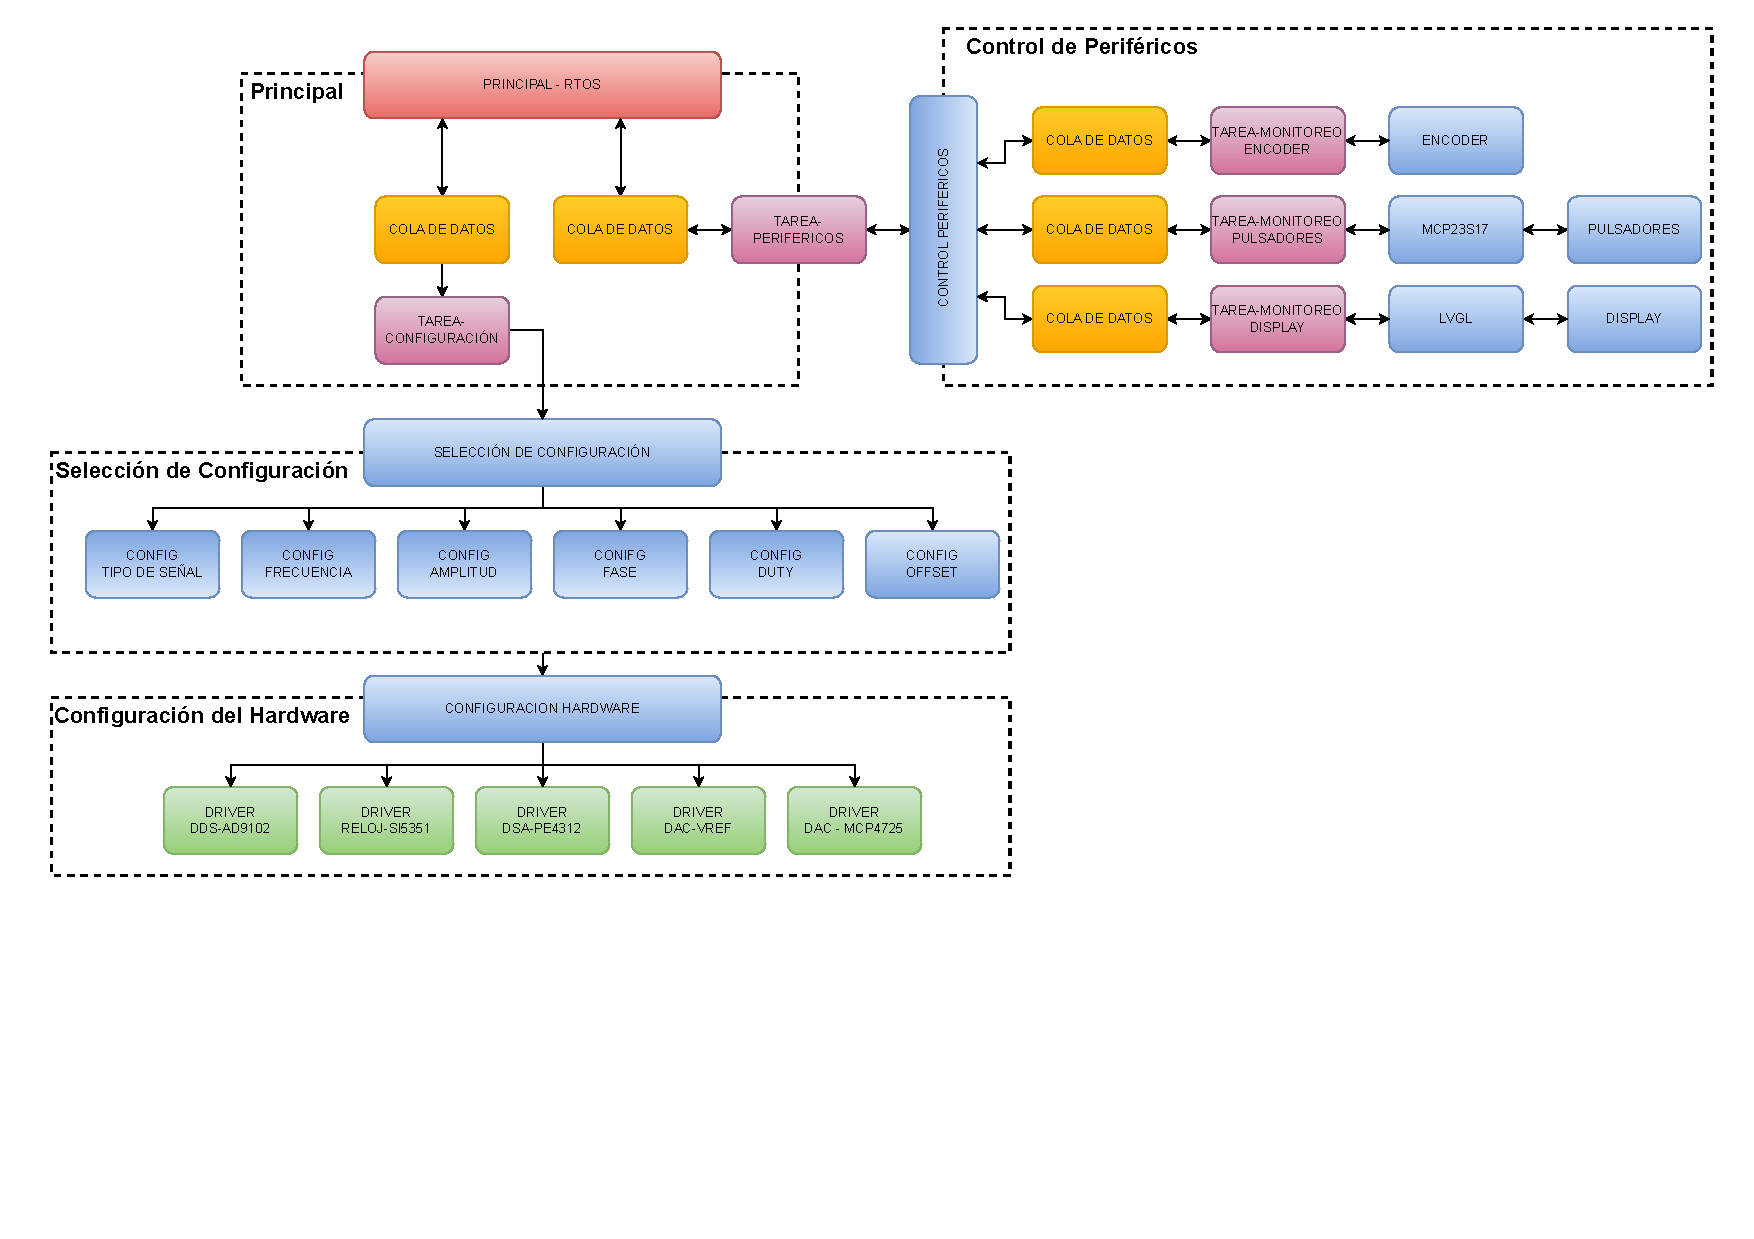
\includegraphics[
	width=\textheight, % usa el "alto" de la página porque está rotada
	clip,
	trim={0cm 5cm 0cm 0cm}
	]{img/Firmware_DB.drawio}
	\caption{Diagrama en bloques del firmware.}
	\label{fig:firmwaredb}
\end{sidewaysfigure}

%\subsubsection{Programación orientada a Objetos}
%La Programación Orientada a Objetos (\textbf{POO}) es un paradigma de programación basado en organizar el software/firmware alrededor de ``objetos'' (datos) y sus comportamientos (métodos), en lugar de funciones lógicas. Reduce errores, promueve la reutilización de código y facilita el mantenimiento de sistemas complejos mediante conceptos como \textit{clases, herencia, encapsulamiento} y \textit{polimorfismo}. 
%
%En el caso de nuestro proyecto la programación orientada a objetos nos va a ser de gran utilidad, porque nos permite poder tener una representación de un ``objeto'' que va a representar algo físico en nuestro circuito. Dicho de otra manera cada objeto va a ser una porción del hardware. Por ejemplo podríamos tener un objeto del tipo \textbf{amplitud}, que cuando el usuario varíe un conjunto de parámetros, esto se vea reflejado en enviar un conjunto de señales al atenuador digital por pasos (DSA), para que la amplitud máxima de la señal de salida varíe. Entonces teniendo este concepto en mente procedemos a la explicación del diagrama en bloques del firmware, Figura \ref{fig:firmwaredb}.

%\subsubsection{Diagrama en bloques del Firmware}
%En este sección se explicarán los elementos más importantes del diagrama en bloques, que pueden visualizarse en la Figura \ref{fig:firmwaredb}.
%
%\paragraph{Principal-RTOS:} Este bloque representa la jerarquía mas alta del código. Se encuentran las configuraciones, declaraciones de objetos y lógica principal. Como se menciona en el nombre puede verse que se va a utilizar un RTOS (a definir), una justificación clara de esto, es que nos permite poder hacer uso de tareas que se ejecuten en forma \textbf{concurrente}. Un ejemplo de estas tareas son la mostradas en color rosa \textbf{TAREA ENCODER}, \textbf{TAREA MONITOREO PULSADORES}, \textbf{TAREA DISPLAY}. Esto nos permite en cierta manera manejar diferentes periféricos de forma paralela, evaluar si hubo cambios o generarlos, si fuese necesario, sin la necesidad de hacer grandes fragmentos de código, dado que son elementos físicos completamente diferentes.
%
%\paragraph{Control de Periféricos:} Su función es actuar como un intermediario entre el mundo externo, en el que se encuentra el usuario y modifica periféricos, y la lógica principal que sería el bloque explicado anteriormente.
%
%\paragraph{Selección de Configuración:} Esta bloque se encarga de procesar la información que ingresa desde la lógica principal, presentada al comienzo, para conmutar entre el tipo de configuración que quiere realizar el usuario. Al final de las explicaciones de lo bloques se presentan un ejemplo globalizar que muestra como cada uno interactúa con el resto, formando un sistema completo.
%
%\paragraph{Configuración del Hardware:} Esta se encarga de recibir un conjunto de valores a modificar y conocimiento de antemano que tipo de configuración es la que está seleccionada, se procede a interactuar con el driver que corresponda, para posteriormente generar el conjunto de señales adecuadas para el circuito integrado correspondiente.
%
%Para tener una visión mas clara de como interactúan todos estos bloques principales se menciona un ejemplo. Supongamos que el usuario quiere modificar la amplitud de salida en el canal 1. Para esto, lo primero que debe hacer es seleccionar dicho canal, pulsando sobre el botón correspondiente. Esta información pasa por el bloque de \textit{Control de Periféricos} que la procesa, agrega algún tipo de parámetro y luego la manda hacia el bloque \textit{Principal}. Este mismo modifica su lógica, informando al siguiente bloque \textit{Selección de Configuración}, cual tipo es seleccionada. Posteriormente el usuario interacciona con el \textit{encoder}, esto se envía por los mismos bloques, ya mencionados, hasta llegar al actual, el cual informa al bloque \textit{Configuración del Hardware} que debe existir un cambio a nivel físico y por lo tanto este mismo actúa en consecuencia sobre el driver correspondiente.


%	\section{Alcance y Objetivos}
La intención de este proyecto consiste en la realización de dicho \textit{Generador de Funciones Arbitrarias} para esto mismo se proponen ciertas características para validar la calidad del dispositivo realizado:

\begin{itemize}
	\item $V_{opp} = $ 10 Vpp.
	\item $V_{in} = $ 85 a 265 VAC.
	\item $I_{o}$ = 20 mA.
	\item 
\end{itemize}
	\newpage

\section{Metodología de ensayo y validación}
La metodología de ensayo propuesta tiene como objetivo verificar el cumplimiento de las especificaciones funcionales y de desempeño del generador de funciones/arbitrario, en el dominio temporal. Se definen el instrumental, las condiciones de medición, los ensayos y los criterios de aceptación.

\subsection{Instrumental y condiciones de medición}
Los ensayos se realizarán bajo condiciones ambientales de laboratorio. Se utilizará el siguiente instrumental:
\begin{itemize}
	\item Osciloscopio con ancho de banda adecuado (idealmente $\geq 5\times$ la frecuencia máxima a evaluar), sondas pasivas y entrada con terminación de 50\,$\Omega$ o alta impedancia según se disponga.
	\item Analizador de espectro (si se dispone) o FFT del osciloscopio para evaluación espectral.
	\item Multímetro TRMS para verificación de amplitud en baja frecuencia.
	\item Cables coaxiales BNC de baja longitud y adaptadores/terminadores adecuados.
\end{itemize}

\subsection{Ensayos funcionales}
Se verificará el correcto funcionamiento de las funciones principales:
\begin{itemize}
	\item \textbf{Generación de formas de onda:} El usuario deberá seleccionar la función de \textit{Tipo de señal} que permitirá cambiar entre las formas de ondas almacenadas previamente senoidal, cuadrada, triangular/rampa, pulso, electrocardiograma, diente de sierra, gausseana, etc.
	\item \textbf{Configuración de parámetros:} El usuario debe seleccionar el parámetro a configurar según corresponda frecuencia, amplitud, offset DC, duty cycle y fase. Con el encoder le permitirá ir variando el valor de cada uno y mediante botones de selección podrá cambiar el multiplicador.
	\item \textbf{Visualización de Configuraciones:} definida a través de la interfaz de visualización que se use (display o PC).
	\item Verificación de interfaz de control (USB/serial/Ethernet) y respuesta a comandos.
\end{itemize}

El resultado satisfactorio de esta etapa radica en la posibilidad de que el usuario/desarrollador pueda manejar de forma correcta las configuraciones mencionadas y que estas se vean claramente representadas en la interfaz de visualización elegida.

%\subsection{Ensayos de frecuencia y resolución}
%Se evaluará la exactitud y resolución de frecuencia mediante puntos de prueba representativos (por ejemplo 1\,kHz, 10\,kHz, 100\,kHz, 300 KHz, 500 KHz, 700 KHz, 1\,MHz, 5\,MHz, 10\,MHz y frecuencia máxima del equipo):
%
%\begin{itemize}
%%	\item \textbf{Error de frecuencia:} $\Delta f = f_\text{medida} - f_\text{programada}$ (si es posible en base a la calidad del instrumental usado).
%	\item \textbf{Resolución efectiva:} menor cambio programable observable en la salida (igual que item anterior).
%\end{itemize}
%
%Como criterio de aceptación se adoptará un error máximo permitido en frecuencia (en ppm o en \%), definido en función de los objetivos del proyecto y del oscilador de referencia utilizado.

\subsection{Ensayos de tipo de señal, frecuencia, amplitud y offset}
En esta sección de presentan todos los tipos de ensayos que van a realizarse, con el fin de darle la mayor caracterización al equipo que se va a realizar. Cada ensayo debe hacerse para cada una de las señales convencionales (senoidal, cuadrada, triangular) y además para alguna arbitraria cargada con una cantidad de muestras definida.

\subsubsection{Ensayo de frecuencia}
Para realizar este ensayo el usuario deberá seleccionar primeramente el tipo de canal que quiere configurar y presionar OK. Luego mediante el encoder rotativo y los botones de cambio de multiplicador, deberá moverlos de acuerdo a la frecuencia que quiera a salida según la tabla proporcionada.

\begin{table}[H]
	\centering
	\label{tab:freq_set_meas}
	\begin{tabular}{|l|c|r|l|}
		\hline
		Tipo de se\~nal & $f_{set}$ & $f_{med}$ & Observaciones \\ \hline
		& 1\,Hz      &  & \\ \hline
		& 10\,Hz     &  & \\ \hline
		& 100\,Hz    &  & \\ \hline
		& 1\,kHz     &  & \\ \hline
		& 10\,kHz    &  & \\ \hline
		& 100\,kHz   &  & \\ \hline
		& 1\,MHz     &  & \\ \hline
		& 3\,MHz     &  & \\ \hline
		& 5\,MHz     &  & \\ \hline
		& 10\,MHz    &  & \\ \hline
		& 15\,MHz    &  & \\ \hline
		& 20\,MHz    &  & \\ \hline
		& 25\,MHz    &  & \\ \hline
	\end{tabular}
	\caption{\textbf{Ensayo frecuencia:} frecuencia configurada vs frecuencia medida ($V_{pp}$ de 20\,V, $V_{off}=0$).}
\end{table}

\subsubsection{Ensayo de amplitud}
Para dicho ensayo el usuario primeramente deberá seleccionar el canal que quiere cambiar la amplitud de salida en Volts de pico a pico o Volts de pico. Una vez seleccionada deberá hacer uso del encoder y botones de cambio de multiplicador para poder ajustar el valor final definido por la siguiente tabla.

\begin{table}[H]
	\centering
	\label{tab:amp_set_meas}
	\begin{tabular}{|l|r|r|r|l|}
		\hline
		Tipo de se\~nal & $V_{pp,set}$ & $V_{pp,med}$ & $V_{off,med}$ & Observaciones \\ \hline
		& 0.2\,V  &  &  & \\ \hline
		& 0.5\,V  &  &  & \\ \hline
		& 1.0\,V  &  &  & \\ \hline
		& 2.0\,V  &  &  & \\ \hline
		& 5.0\,V  &  &  & \\ \hline
		& 10.0\,V &  &  & \\ \hline
		& 15.0\,V &  &  & \\ \hline
		& 20.0\,V &  &  & \\ \hline
	\end{tabular}
	\caption{\textbf{Ensayo amplitud:} amplitud configurada vs amplitud medida (frecuencia 10\,kHz, $V_{off}=0$).}
\end{table}

\subsubsection{Ensayo de offset}
El procedimiento es el mismo que los ensayos anteriores, seleccionando en este caso el boton de cambio de offset o señal de DC.

\begin{table}[H]
	\centering
	\label{tab:offset_set_meas}
	\begin{tabular}{|l|r|r|r|l|}
		\hline
		Tipo de se\~nal & $V_{off,set}$ & $V_{off,med}$ & $V_{pp,med}$ & Observaciones \\ \hline
		& -5.0\,V &  &  & \\ \hline
		& -4.0\,V &  &  & \\ \hline
		& -3.0\,V &  &  & \\ \hline
		& -2.0\,V &  &  & \\ \hline
		& -1.0\,V &  &  & \\ \hline
		& -0.5\,V &  &  & \\ \hline
		& 0.0\,V  &  &  & \\ \hline
		& +0.5\,V &  &  & \\ \hline
		& +1.0\,V &  &  & \\ \hline
		& +2.0\,V &  &  & \\ \hline
		& +3.0\,V &  &  & \\ \hline
		& +4.0\,V &  &  & \\ \hline
		& +5.0\,V &  &  & \\ \hline
	\end{tabular}
	\caption{\textbf{Ensayo offset:} offset configurado vs offset medido (frecuencia 10\,kHz, $V_{pp}$ fijo).}
\end{table}

\subsubsection{Ensayo de planitud}
A diferencia de los ensayos anteriores el usuario ahora deberá configurar tanto la amplitud en un valor definido (preferentemente el máximo) e ir incrementando la frecuencia y visualizar la tensión de salida máxima. Esto se hace con el fin de poder ver que tan estable es la salida frente a diferentes frecuencias y a su vez las limitaciones propias del equipo. Además al hacerlo tanto para alta impedancia como baja impedancia las condiciones serán distintas ya que en baja impedancia la exigencia será mucho mayor.

\begin{table}[H]
	\centering
	\label{tab:sine_flatness_basic}
	\begin{tabular}{|c |r| l|}
		\hline
		$f$ & $V_{pp,med}$ & Condición (Hi-Z / 50$\Omega$) \\
		\hline
		1\,kHz    &  & \\ \hline
		10\,kHz   &  & \\ \hline
		100\,kHz  &  & \\ \hline
		1\,MHz    &  & \\ \hline
		5\,MHz    &  & \\ \hline
		10\,MHz   &  & \\ \hline
		20\,MHz   &  & \\
		\hline
		25\,MHz   &  & \\
		\hline
	\end{tabular}
	\caption{\textbf{Ensayo senoidal:} amplitud medida vs frecuencia.}
\end{table}

\subsubsection{Ensayos específicos}
Incluyen todos los ensayos que depende exclusivamente del tipo de señal.

\begin{table}[H]
	\centering
	\label{tab:square_duty_rise}
	\begin{tabular}{|c| r| r| r| c| r| r| l|}
		\hline
		$f_{set}$ & $f_{med}$ &
		$V_{pp,set}$ & $V_{pp,med}$ &
		Duty$_{set}$ & Duty$_{med}$ &
		$t_r$ / $t_f$ &
		Obs. \\
		\hline
		1\,kHz   &  & 1.0\,V &  & 50\% &  &  & \\ \hline
		100\,kHz &  & 1.0\,V &  & 50\% &  &  & \\ \hline
		1\,MHz   &  & 1.0\,V &  & 50\% &  &  & \\
		\hline
	\end{tabular}
	\caption{Ensayo específico: señal cuadrada (duty y tiempos).}
\end{table}


%\subsection{Integridad de señal en el dominio temporal}
%Para cada forma de onda, especialmente a frecuencias elevadas, se evaluará:
%
%\begin{itemize}
%	\item \textbf{Para senoidal:} ruido observable, estabilidad y distorsión.
%	\item \textbf{Para cuadrada/pulso:} tiempos de subida y bajada (10--90\%), overshoot/undershoot para ciertas frecuencias seleccionadas, duty real versus duty programado.
%\end{itemize}
%
%Dado que se trata de un proyecto final a nivel educativo y no un dispositivo comercial, la validación de la etapa será en función de los resultados obtenidos.

%\subsection{Ensayos espectrales (armónicos, THD, SFDR)}
%Se caracterizará la calidad espectral mediante FFT del osciloscopio o analizador de espectro. Para una senoidal (por ejemplo 1\,MHz y 10\,MHz) se evaluará:
%
%\begin{itemize}
%	\item Niveles de armónicos (2º, 3º, etc.).
%	\item THD o THD+N (si el instrumento lo permite).
%	\item SFDR: diferencia entre el tono fundamental y el mayor espurio.
%\end{itemize}
%
%Se verificará que el contenido espectral sea consistente con la forma cargada y que no existan espurios dominantes no esperados. En caso de aparecer mencionarlos y dar una breve justificación.
%	\section{Instrumental de trabajo}
Para el desarrollo, integración y validación del prototipo se utilizará el siguiente instrumental y equipamiento de laboratorio:

\begin{itemize}
	\item \textbf{PC de desarrollo:} estación de trabajo con entorno de compilación, programación y depuración del firmware, control de versiones y documentación.
	\item \textbf{Fuente de alimentación de laboratorio:} fuente regulable con limitación de corriente para pruebas seguras del prototipo y de sus rieles de alimentación.
	\item \textbf{Osciloscopio digital:} para verificación de formas de onda, medición de amplitud, offset, tiempos de transición y jitter. Se emplearán sondas pasivas y, cuando corresponda, terminación de 50\,$\Omega$.
	\item \textbf{Multímetro digital TRMS:} para mediciones de tensión y corriente en continua y alterna, y verificación de rieles de alimentación.
	\item \textbf{Analizador de espectro / FFT de osciloscopio:} para caracterización espectral (armónicos, espurios) y estimación de métricas como THD y SFDR, si se dispone.
	\item \textbf{Cargas y terminaciones:} resistencias de potencia, terminaciones coaxiales de 50\,$\Omega$, y condición High-Z (1\,M$\Omega$) para ensayos comparativos.
	\item \textbf{Cables y conectividad:} cables coaxiales BNC cortos, adaptadores, conectores, pinzas y puntas de prueba para minimizar errores de medición.
	\item \textbf{Herramientas de montaje y retrabajo:} estación de soldado, estación de aire caliente, flux, estaño, lupa/microscopio, y consumibles para ensamblado SMD.
	\item \textbf{Instrumental para verificación de componentes}.
\end{itemize}

En particular se va a utilizar el osciloscopio \textbf{OWON VDS1022I}. Puede verse una imagen ilustrativa a continuación.

\begin{figure}[H]
	\centering
	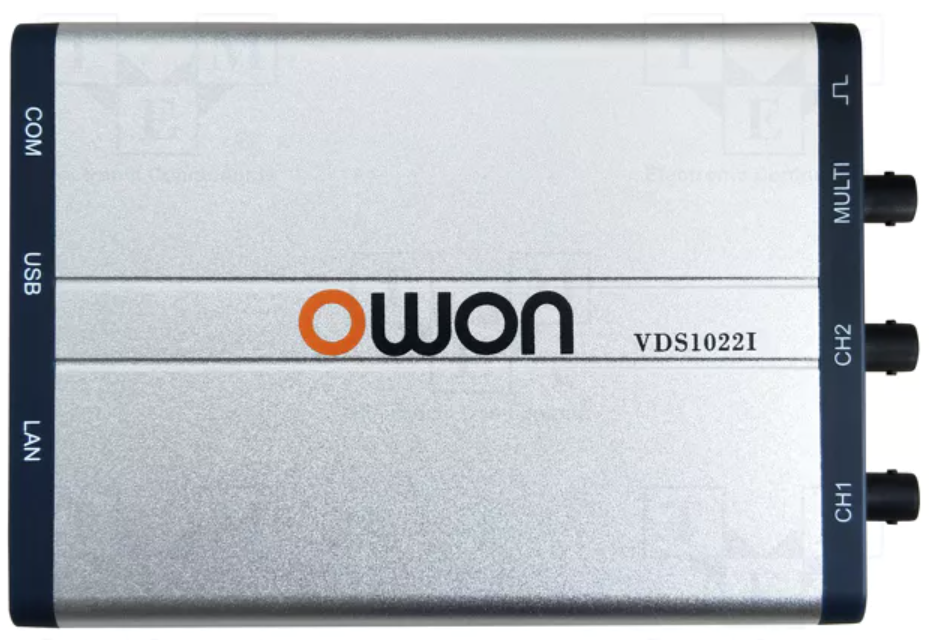
\includegraphics[width=0.7\linewidth]{Comparacion/img/owon_vds1022i}
	\caption{Osciloscopio OWON VDS1022I.}
	\label{fig:owonvds1022i}
\end{figure}

\paragraph{OWON VDS1022I (osciloscopio USB aislado para PC):}
Es un osciloscopio digital basado en PC, de \textbf{2 canales} con \textbf{aislación por USB}, orientado a mediciones generales y portabilidad.

\begin{itemize}
	\item \textbf{Canales:} 2 + 1 (entrada externa / multifunción). 
	\item \textbf{Ancho de banda analógico:} 25\,MHz.
	\item \textbf{Tasa de muestreo en tiempo real:} 100\,MSa/s.
	\item \textbf{Resolución vertical (ADC):} 8\,bits (2 canales simultáneos).
	\item \textbf{Memoria / record length:} 5\,kpts.
	\item \textbf{Base de tiempos:} 5\,ns/div a 100\,s/div (pasos 1--2--5).
	\item \textbf{Sensibilidad vertical:} 5\,mV/div a 5\,V/div.
	\item \textbf{Impedancia de entrada:} 1\,M$\Omega$ en paralelo con $\sim$10\,pF.
	\item \textbf{Acoplamiento de entrada:} DC, AC y GND.
	\item \textbf{Tensión máxima de entrada:} hasta 400\,V (pico a pico), según condición de medición/probador.
	\item \textbf{Modos de adquisición:} sample, peak detect y average.
	\item \textbf{Disparos (trigger):} edge, pulse, video, slope y alternate; modos auto/normal/single.
	\item \textbf{Funciones matemáticas:} suma, resta, multiplicación, división, inversión y FFT; vistas FFT y X--Y.
	\item \textbf{Interfaz:} USB 2.0 con \textbf{aislación} (menor interferencia y protección de la PC).
	\item \textbf{Alimentación:} por bus USB (no requiere fuente externa).
\end{itemize}
%	\section{Avances realizados}
En esta sección se presentan los avances que fueron realizados durante el proceso de desarrollo del anteproyecto de forma preliminar. Dentro de estos avances se encuentra el diseño de la \textbf{placa de Alimentación} a través del programa de diseño \textbf{Altium} que puede verse en la Figura \ref{fig:placaalimentacion} y \ref{fig:placaalimentacionvuelta}. También se fue realizando el diseño de la \textbf{placa de Control} y la \textbf{placa de panel Frontal}, quedando como parte del trabajo una vez aprobado el anteproyecto terminarlas.

\begin{figure}[H]
	\centering
	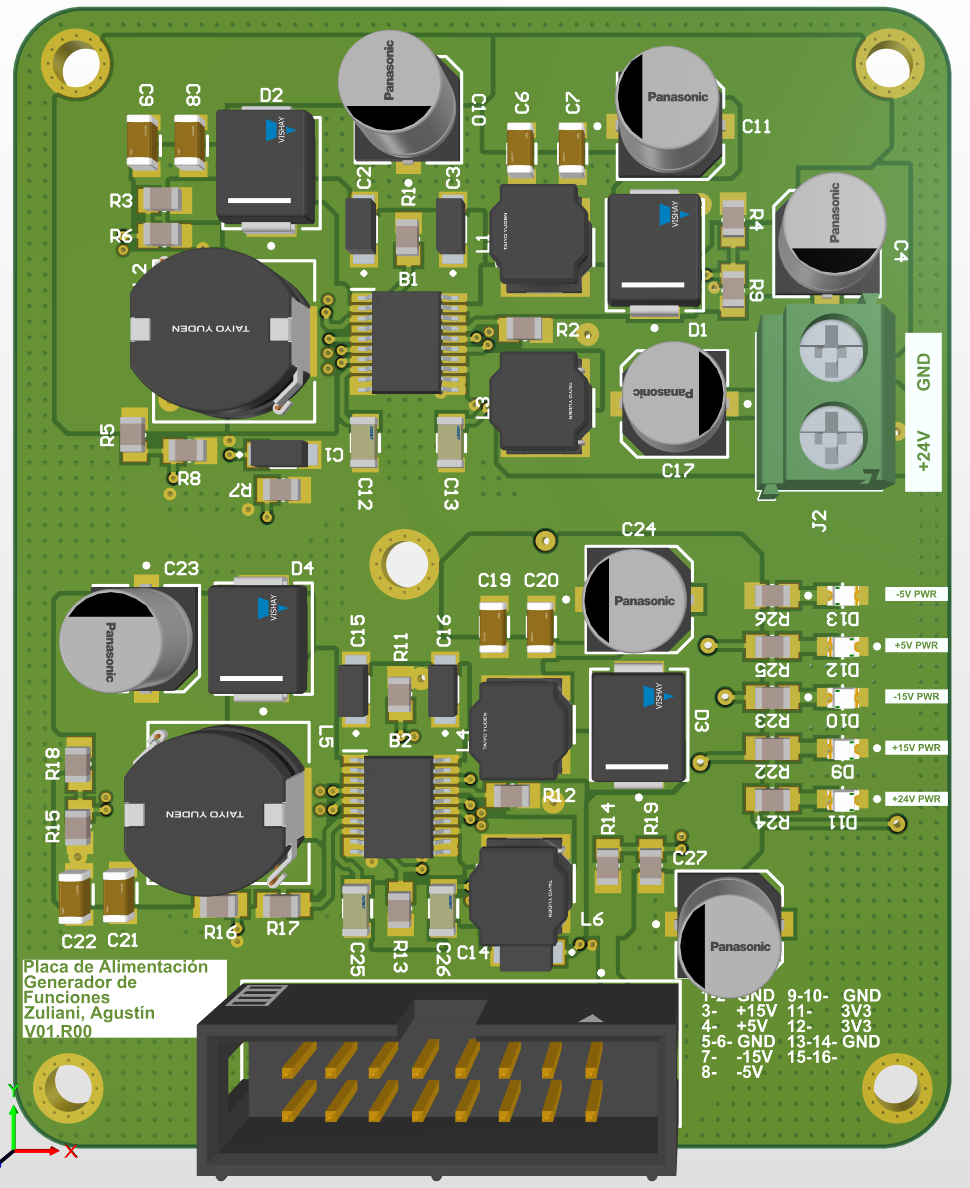
\includegraphics[width=0.5\linewidth]{Conclusion/img/placa_alimentacion}
	\caption{Placa de Alimentación diseñada V01.R00 del lado TOP.}
	\label{fig:placaalimentacion}
\end{figure}

\begin{figure}[H]
	\centering
	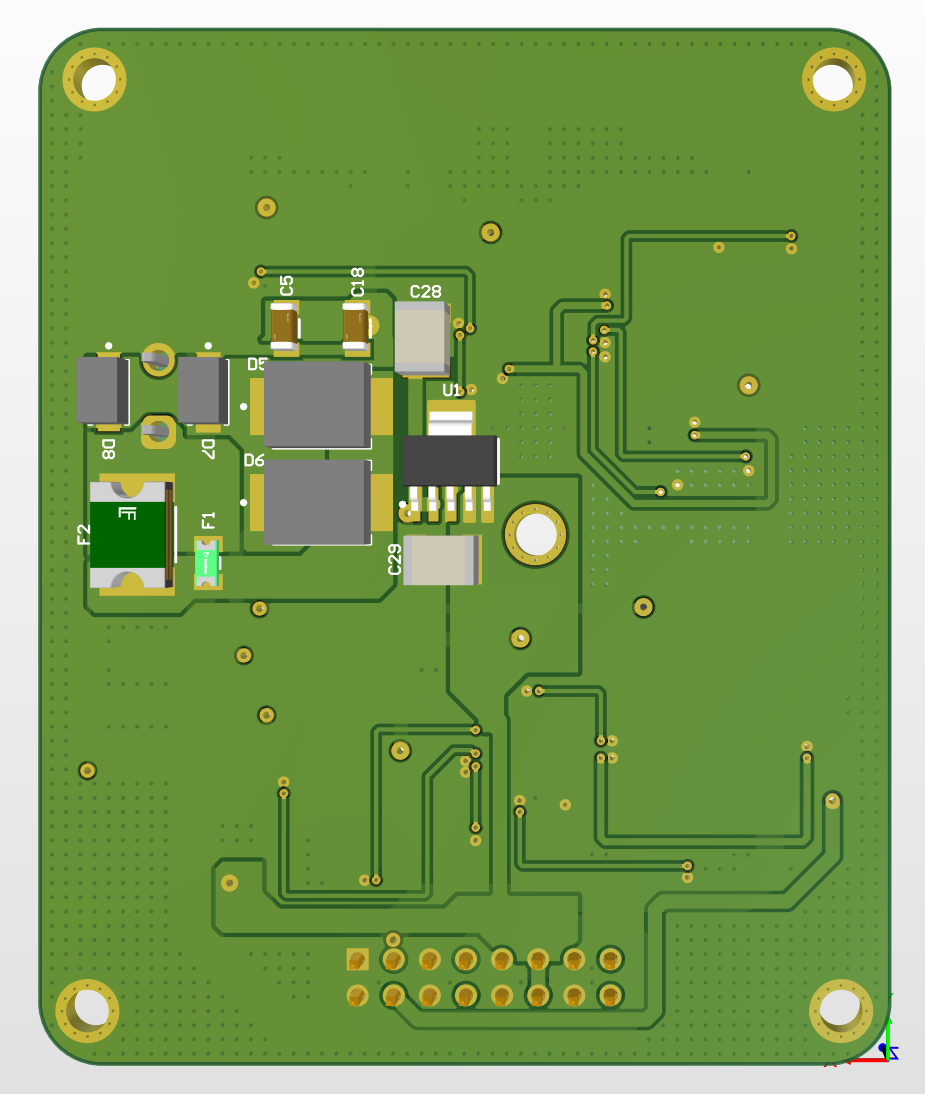
\includegraphics[width=0.5\linewidth]{Conclusion/img/placa_alimentacion_vuelta}
	\caption{Placa de Alimentación V01.R00 del lado Bottom.}
	\label{fig:placaalimentacionvuelta}
\end{figure}

%	\section{Mejoras a futuro}
Para finalizar el anteproyecto se presentan esta última sección que mencionan todas aquellas cosas que se quieren realizar pero que por un motivo u otro quedan fuera del alcance.

\subsection{Diseño de GUI para usuario}
Una GUI es una interfaz gráfica que permite al usuario poder manipular el dispositivo conectado desde la PC. Esta misma haría uso del conector Ethernet que se encuentra dentro del propio dispositivo, el mismo que permite el uso para laboratorio remoto. La idea detrás de este GUI sería lograr que el usuario pueda realizar las mismas configuraciones que venía haciendo para la generación de la forma de onda, pero además permita cargar tablas de muestras para una nueva forma arbitraria definida por el propio usuario.

\subsection{Implementación de funcionalidades/contador}
A modo de comparar con el equipo proporcionado por FeelElec FY6900 queda como futura mejora la implementación de funcionalidades extras que permitan darle un mayor valor al propio instrumento realizado, así como también la implementación de un contador digital de frecuencia que puede realizarse con una FPGA.

\subsection{Mejora del display con LVGL}
La idea de esta mejora consiste en la utilización de un nuevo display (ya contemplado en el diseño del hardware) que permita el uso de librerías como LVGL, de forma que brinde al usuario una mejor representación gráfica.

\subsection{Diseño de una carcasa y frente adecuados}
Debido a la longitud del proyecto algunas cosas como la presentación final del instrumento no sean adecuadas, la idea de esta mejora consiste en realizar una carcasa y frente a nivel industrial, de forma que el instrumento pueda ser comerciable y adquirido por cualquier usuario.

	
	\newpage
	
	\bibliographystyle{plain}
	\bibliography{bibliografia}
	
\end{document}